%--------------------------------------------------------------------------------------%--------------------------------------------------------------------------------------
%
%  Global settings, dont change it! (excapt additional \usepackage commands)
%  Always use PDFLatex!
%
%--------------------------------------------------------------------------------------%--------------------------------------------------------------------------------------
\documentclass[a4paper, 11pt, oneside, BCOR1cm,toc=chapterentrywithdots]{scrbook}

\usepackage[pdftex]{graphicx}           % use for pdfLatex
\usepackage{makeidx} % f\"{u}r Benutzung des Befehls \printindex
\usepackage[colorlinks=false]{hyperref}
\usepackage[nottoc]{tocbibind}
\usepackage{blindtext}
\usepackage{subfigure} 
\usepackage{acronym}
%\usepackage{algorithm}
\usepackage[ruled,vlined,linesnumbered]{algorithm2e}
%\usepackage{algorithmic}
%\usepackage{algpseudocode}
\usepackage{float}
\usepackage{cite}
\usepackage{tabularx}
\usepackage{booktabs}
\usepackage{amssymb}
\usepackage{wrapfig}
\usepackage{enumitem}
\usepackage{amsmath}
\usepackage{listings}
\usepackage{longtable}
\usepackage{makecell}
\usepackage[skip=3pt]{caption}
\usepackage{pgfplots}
\usepackage{etoolbox}
\usepackage{setspace}
\usepackage[toc,page]{appendix}

\newtheorem{Def}{Definition}[section]


\hypersetup{%
bookmarksnumbered=true, hyperindex=true,
%
%Im Acrobat Reader Subtitel 1. Ebene anzeigen
bookmarksopen=true, bookmarksopenlevel=1,
%
pdfborder=0 0 0 % Keine Box um die Links!
}

% --------------------------------------------------------------
% Force Tables and List to be added in Table of Content
% --------------------------------------------------------------

\renewcommand*{\tableofcontents}{%
  	\begingroup
  	\tocsection
  	\tocfile{\contentsname}{toc}
  	\endgroup
}
\renewcommand*{\listoffigures}{%
  	\begingroup
  	\tocsection
  	\tocfile{\listfigurename}{lof}
  	\endgroup
}
\renewcommand{\listoftables}{
	\begingroup
	\tocsection
	\tocfile{\listtablename}{lot}
	\endgroup
}
\begin{document}

%--------------------------------------------------------------------------------------%--------------------------------------------------------------------------------------
%
%  Here starts the userspace !
%
%--------------------------------------------------------------------------------------%--------------------------------------------------------------------------------------

%--------titlepage
\begin{titlepage}

{
    \begin{flushright}
        \raisebox{-1ex}{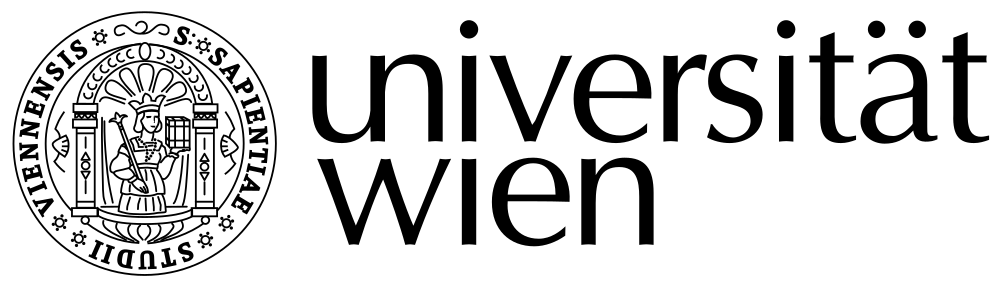
\includegraphics[scale=0.15]{Logo.png}}\\
    \end{flushright}
    \vspace{1.5cm}
}

\begin{center}
\LARGE{\textbf{MASTERARBEIT / MASTER'S THESIS}}\\
\vspace{1.5cm}

\small{Titel der Masterarbeit / Title of the Master's Thesis}\\
\Large{\textbf{"Automatic Generation and Translation of Process Collaboration Models to BPMN/XML"}}\\ 
\vspace{1.5cm}
\small{verfasst von / submitted by}\\
\large{Frederik Bischoff BSc }\\
\vspace{1.5cm}
\small{angestrebter akademischer Grad / in partial fulfilment of the requirements for the degree of}\\
\large{Diplom-Ingenieur (Dipl.-Ing.)}\\
\end{center}
\vspace{1.25cm}
\small{Wien, 2018 / Vienna 2018}\\
\vspace{1.25cm}\\
\begin{tabbing}
Studienkennzahl lt. Studienblatt / \hspace{2cm} \= A 066 926\\
degree programme code as it appears on\\
the student record sheet:\\[0.5cm]
Studienrichtung lt. Studienblatt / \> Masterstudium Wirtschaftsinformatik\\
degree programme as it appears on\\
the student record sheet:\\[0.5cm]
Betreut von / Supervisor: \> Univ.-Prof. Dipl.-Math. Dr. Stefanie Rinderle-Ma\\
\end{tabbing}
\end{titlepage}


%---------------------------------------------------------
% Table of Contents, List of figures, List of Tables
%---------------------------------------------------------
\begin{spacing}{0.95}
\tableofcontents
\end{spacing}

%---------------------------------------------------------
% Here starts the real work
%---------------------------------------------------------
\makeatletter
\patchcmd{\scr@startchapter}{\if@openright\cleardoublepage\else\clearpage\fi}{}{}{}
\makeatother

\vspace{-0.4cm}
\chapter{Introduction}
In the research field of business process models and techniques, researchers can only rely on a repository of centralized, intra-organizational processes to support their work. But regarding decentralized, cross-organizational models, they face the problem that there is a lack of available model examples. Within the scope of this work, this lack is aimed to be tackled. Thereby, the main objective is to build a repository of distributed and collaborative process models by developing and implementing an automatic generation process for business process collaborations. The generation process must thereby ensure soundness, consistency and compatibility of the resulting models. Additionally, it should also allow the generation of models which comply to imposed compliance rules. At last, to ensure the executability of the auto-generated models by process engines, an additional goal of this work is to develop a transformation of the utilized RPST\footnote{Refined Process Structure Tree } representation to BPMN\footnote{Business Process Model and Notation - http://www.bpmn.org/}. These requirements ensure that the repository can then be used for further research, such as change management or process mining of collaborative processes. Based on those objectives, the following research questions are derived:

\begin{itemize}
\item \textit{RQ-1}: How to build a repository of collaboration process models that can be used as support for further research in this field?
\item \textit{RQ-2}: How to ensure that the resulting process models in this repository are correct in terms of consistency, compatibility and compliability? Which process flow perspectives and compliance rule patterns should be supported regarding compliability? 
\item \textit{RQ-3}: How to transform a collaborative process represented as an RPST into an executable form?
\end{itemize}

This work is part of the CRISP\footnote{http://gruppe.wst.univie.ac.at/projects/crisp/} project (ICT15-072) funded by the Vienna Science and Technology Fund (WWTF). The implementation of the prototype is integrated in an already existing framework. The main research within the project is to analyze flexibility and adaptivity of collaborative business processes at design time as well as at runtime. Regarding consistency and correctness of collaborative business processes, the propagation of a process change over all process participants is one of the main challenges the project tries to tackle. Furthermore, the impact of compliance rules imposed on collaborative business scenarios is analyzed as well as the issue of ensuring business compliance by considering the privacy and autonomy of the involved business partners.\\

This work is structured as followed. First, a brief overview of related work is given in Chapter \ref{chap:relwork}, followed by an introduction into process collaborations represented in BPMN by explaining the different model views in Chapter \ref{chap:theo}. Then the concept of the automatic collaboration process generator is introduced in Chapter \ref{chap:conception}. Thereby the approach, the possibility of influencing the outcome and the therefor necessary components are explained. Afterwards, in Chapter \ref{chap:impl}, the adaption of the RPST for the internal process model representation is explained as well as the class structure and data models of the implemented components. The performance of the implemented generation process depending on different parameter settings is then examined in Chapter \ref{chap:analysis}. Finally, the work is concluded in Chapter \ref{chap:concl}.  % Load Data from File intro.tex
\vspace{-0.4cm}
\chapter{Related Work}
\label{chap:relwork}
This work focuses on the generation of collaborative business process models. Thus, the thereby introduced method of generating processes randomly can be compared with work that also generate business process models but differ from the input source of generation and it's algorithm. In comparison to the purpose of this work, which is building a repository of process collaborations to facilitate further research, they mainly have the goal to simplify the process of business process modeling by reducing the time for process acquisition and also generation. At the end, a similar research is introduced which also follows an approach of random process generation with the goal to facilitate further research with process examples.\\
There is research on generating processes from natural language \cite{natlang1}\cite{natlang2}. In \cite{natlang1}, Friedrich et al. introduced an approach to generate BPMN process models from natural language texts by utilizing syntax parsing and semantic analyzing mechanism in combination with anaphora resolution\footnote{Resolving what a pronoun or noun refers to.}. The result of the parsing algorithm is a declarative model that includes the extracted actions, actors and their dependencies. This model then serves as basis for the BPMN model composition. Compared to that, Krzysztof et al. introduced an transformation approach for structured natural language in form of SBVR\footnote{Semantics of Business Vocabulary and Business Rules} in \cite{natlang2}.\\
There are also approaches which generate BPMN models on the basis of UML\footnote{Unified Modeling Language} use cases \cite{relUML1} \cite{relUML2} or sequence diagrams \cite{relUML3}.\\
Another interesting, recent research focuses on the generation of process models based on constraint programming \cite{relCP}. Therein, Wisniewski et al. introduced an approach which uses semi-structured information about process activities along with their execution conditions as input for a constraint satisfaction problem (CSP). On the basis of this CSP, a constraint solver generates synthetic execution logs of all valid execution sequences. At last, the BPMN model is generated with the aid of process mining techniques. Their approach is similar to the one introduced in this work. The conceived model generation algorithm in this work also takes user defined dependencies between tasks (see Chapter \ref{sec:conception_compliance}) into account.\\
In \cite{relPLG}, Burattin also introduced a tool for generating BPMN process models randomly. In contrast to this work, which focuses on process collaborations, the tool only supports basic process models with the components task, exclusive and parallel gateways. The tool also supports user-defined parameters to influence the model outcome in terms of number of node types and level of branching. It is also possible to import existing models in order to evolve them. But in contrary to this work, it's main purpose is less the generation of random process models than the combination with the possibility to simulate the processes in order to obtain execution logs for testing process mining algorithms.
\vspace{-0.4cm}
\chapter{Process Collaborations in BPMN}
\label{chap:theo}
This chapter provides the basics of business process collaborations, represented in BPMN. In BPMN, collaborative processes are represented from different perspectives, whereas each perspective is represented by a different BPMN model type. In the following, the different model types and their represented perspective are explained with the help of a collaborative business process example.

\subsubsection{Private Model}
The private model is modeled from the perspective of a single participant of a collaborative process. In a collaborative scenario, it describes the complete internal business logic of one partner as well as the messages exchanged with other partners. Activities which are only for the participant are called \textit{private activities}, whereas activities which involve participation of other partners are called \textit{public activities}.\\

\begin{figure}[H]
\centering
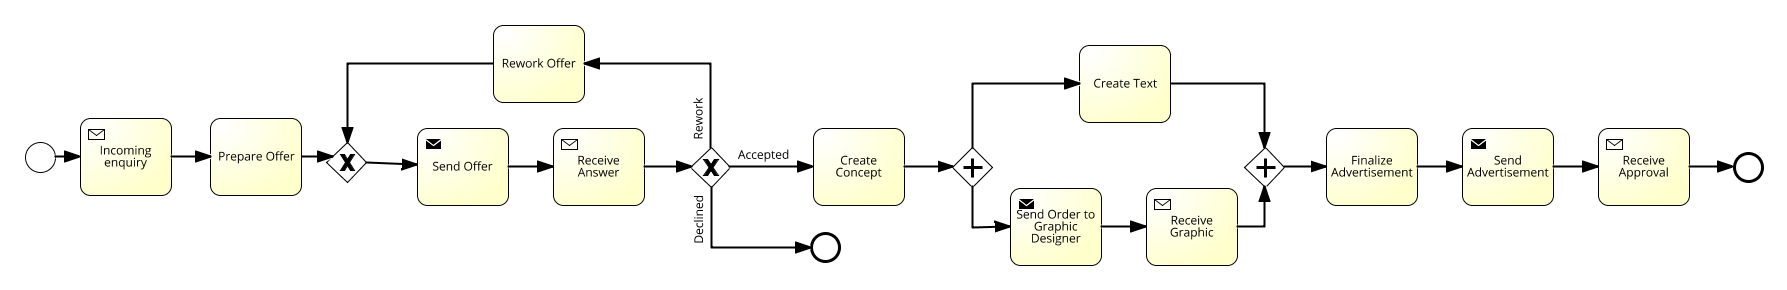
\includegraphics[width=0.9\textwidth]{src/images/private_process_agency.png}
\caption{Private Model Example}
\label{fig:privateModel}
\end{figure}

For example, in the private model shown in Figure \ref{fig:privateModel}, the task \textit{Create Concept} represents a private activity, whereas the task \textit{Send Offer}, involves message exchange with another participant and therefore represents a public activity. A private model is a process model in the classical sense. It's fundamental modeling objects are unchanged since BPMN 1.0. Is a private process modeled and attributed in detail, it also represents an executable process that can be executed by a process engine.

\subsubsection{Public Model}
The public model is also modeled from the perspective of a single participant of a collaborative process. It is a reduced view on the private model of a partner. It can also be described as a projection of the whole collaboration process focusing on one participant. It only includes public activities, involving message exchange with other partners. Private activities which are not relevant for other partners and which don't want be to be shared with the partners are omitted deliberately. Figure \ref{fig:publicModel} shows the corresponding of the already introduced private model. 

\begin{figure}[H]
\centering
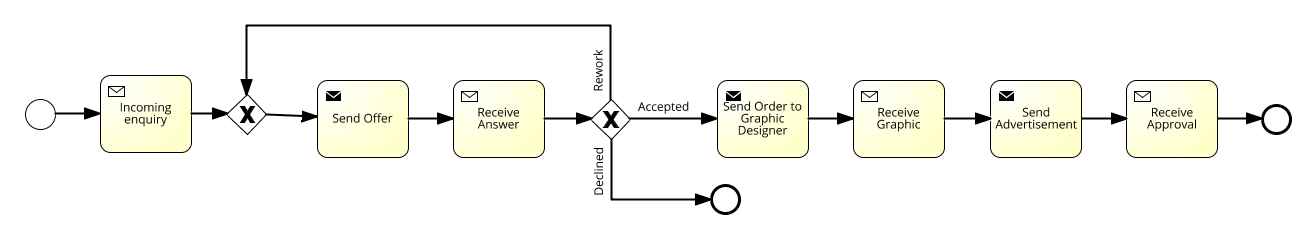
\includegraphics[width=0.9\textwidth]{src/images/public_process_agency.png}
\caption{Public Model Example}
\label{fig:publicModel}
\end{figure}

\subsubsection{Collaboration Model}
The collaboration model is the interconnection between the public models of all participants. The thereby formed model gives a holistic view on the collaborative process and does not focus on one partner. Each partner is represented as a pool and the message exchange between them is shown by a message flow that connects two public activities or just the pools. Figure \ref{fig:collabModel} shows an example collaboration model.

\begin{figure}[H]
\centering
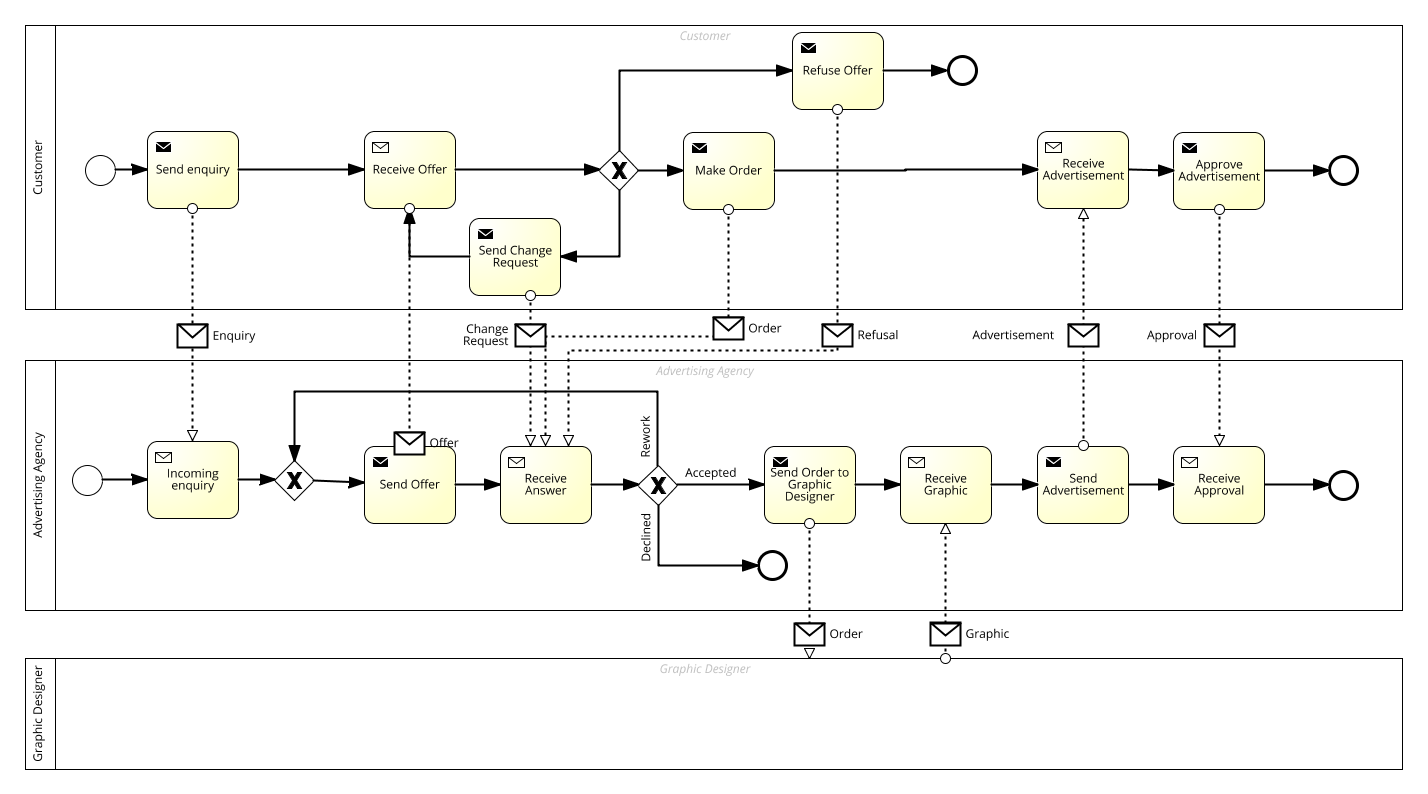
\includegraphics[width=0.9\textwidth]{src/images/collab_advertisement.png}
\caption{Collaboration Model Example}
\label{fig:collabModel}
\end{figure}

Each partner's public process is modeled inside a pool. It is also allowed for a process to not include the public model inside an participant's pool. If a pool contains a process, it is called a "white box". If a pool is empty, it's called a "black box". For Example in figure \ref{fig:collabModel} the pools of the partners \textit{Customer} and \textit{Advertisement Agency} are modeled as "white box" and the pool of the \textit{Graphic Designer} as a "black box" \cite{BPMN20}.

\subsubsection{Choreography Model}
The choreography model is available since BPMN 2.0 and focuses solely on the sequence of message exchanges between the partners. Each message exchange is represented as an interaction with an initiating 
partner, a receiving partner (shaded in grey) and the message exchanged. In contrast to the collaboration model, which also focuses on the message flow, the choreography model additionally displays the exact sequence flow (i.e. conditional message flows or parallel message flows), which is not always evident form the former (i.e. black box pools).

\begin{figure}[H]
\centering
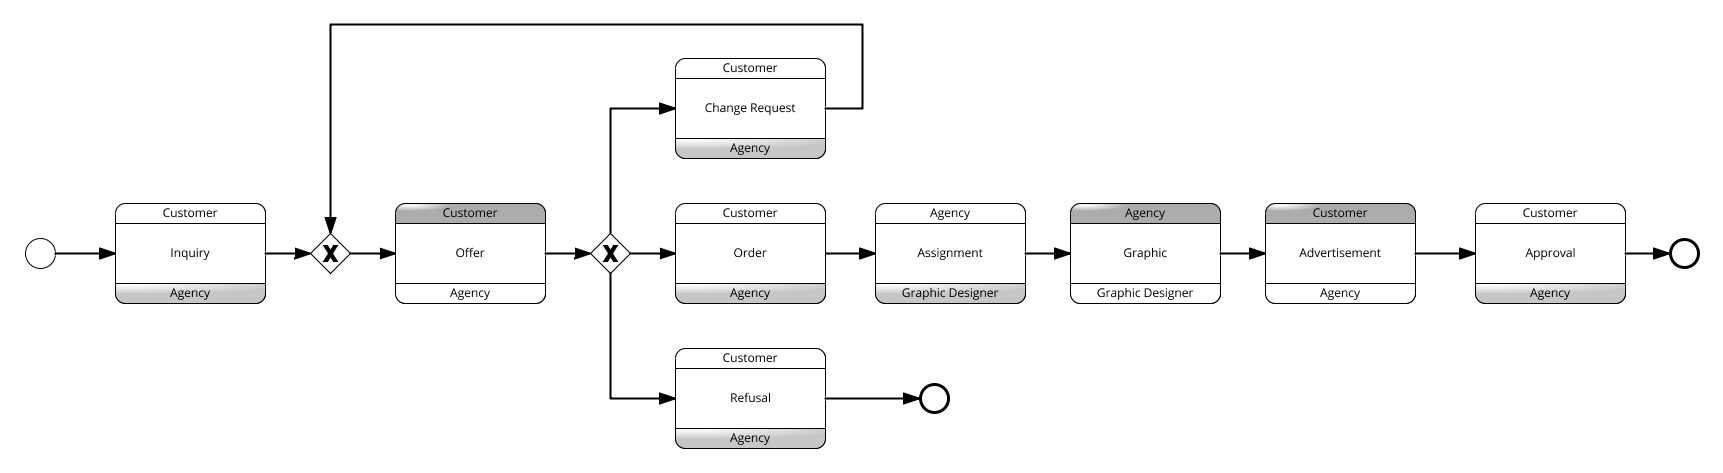
\includegraphics[width=0.9\textwidth]{src/images/choreo_advertisement.png}
\caption{Choreography Model Example}
\label{fig:choreoModel}
\end{figure}
\vspace{-0.6cm}
\chapter{Conception}
\label{chap:conception}
\renewcommand{\lstlistingname}{Example}

The previous chapter covered the necessary background information on business process collaborations represented in BPMN and their different perspectives. In this chapter, the conception of the automatic process collaboration generator is introduced.

\section{Approach}

As already mentioned in Chapter \ref{chap:theo}, a process collaboration involving several partners can be modeled from different perspectives (partner or global) through the use of different model types. The process collaboration generator, implemented in the context of this work, generates all three different model types as the output. In general, there exist two different approaches to build a process collaboration with all the described models \cite{sabrina1174}. In the \textit{top-down approach}, first the choreography model is build, then the public and private models of each partner are derived and defined consistently. In comparison, in the \textit{bottom-up approach}, each partner has already defined a private and public process. Then, the choreography model is constructed by connecting the public models via message exchange. \par
The automatic generator, presented in this work, follows the \textit{top-down approach}, by first generating the choreography model and then deriving the collaboration, public and private models from it. Thereby, each interaction (choreography task) of the choreography model is converted into a send and receive task and then added to the involved partners processes, to build their public process models. In turn, each private model is derived from its corresponding public model by enriching the public model with abstract private tasks. The collaboration model is then built by composing the partner's public processes into one model.\\

\begin{wrapfigure}[11]{r}{0.5\textwidth}
\vspace{-0.5cm}
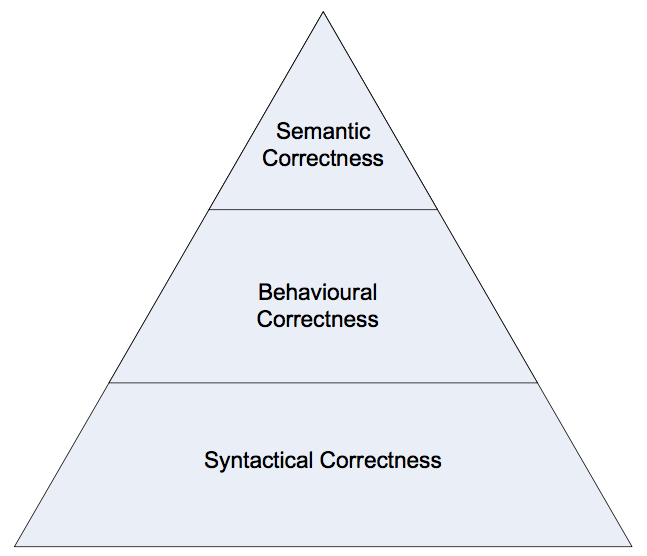
\includegraphics[width=0.9\linewidth]{src/images/correctness_levels.png}
\caption{Pyramid of Business Process Model Correctness\\(Source: \cite{sabrina848})}
\label{fig:bpm_correctness}
\end{wrapfigure}

Generally, when defining business process models, three levels of correctness need to be considered and satisfied by the models:\\

\textit{Syntactical Correctness} is defined by the underlying BPMN meta model and refers to the correct use and composition of the corresponding model elements. Syntactical constraints for example include the fact that any model must at least  have one start and one end event,\\ 
as well as  that flow  objects (e.g. tasks,\\ 
gateways, events) can only be connected\\
by control flow edges \cite{sabrina848}. \\

\textit{Behavioral Correctness} constitutes that a process model must be executable and therefore free of deadlocks or lifelocks. It assumes that the model is syntactically correct, because the behavior of a syntactical incorrect model is undefined. Regarding collaborative, cross-organizational processes, it is also required that the composition of the involved public models is compatible. For example, this means, that for every message that is send, a corresponding partner must be able to receive it \cite{sabrina1174, sabrina848}. \\

\textit{Semantic Correctness} means that the a process model must comply with imposed compliance rules \cite{sabrina848}. Thereby it must be differentiated between \textit{local} and \textit{global compliance rules}. \textit{Local compliance rules} constrain the private process of a partner, whereas \textit{global compliance rules} constrain the interaction between multiple partners \cite{sabrina1174}. In this work, only \textit{global compliance rules} are considered to constrain the choreography model.

\begin{figure}[H]
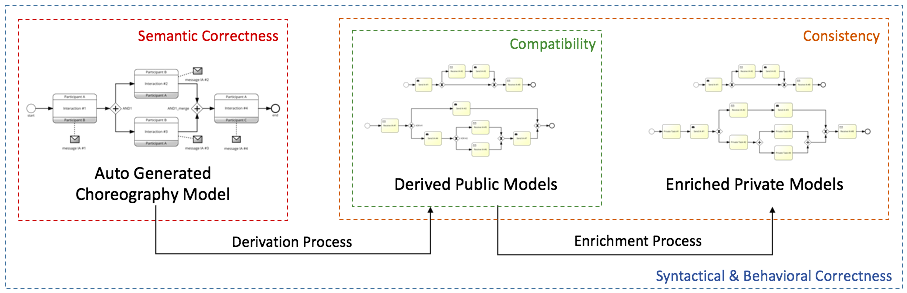
\includegraphics[width=1\textwidth]{src/images/conception_approach.png}
\caption{Top-Down Approach}
\label{fig:topdownapproach}
\end{figure}

All three correctness levels are considered by the proposed algorithm for implementing an automatic process generator. The algorithm ensures that only model specific flow objects are used to build the processes and that they are connected appropriately (syntactical correctness). It also guarantees the absence of deadlocks and lifelocks (behavioral correctness) and offers the possibility to define global compliance rules (see Chapter \ref{sec:conception_compliance}), to which the generated collaboration should comply (semantic correctness). Deriving all models from the before generated choreography model offers also the advantage, that if the deriving process is implemented correctly, it already ensures \textit{consistency} and \textit{compatibility} between the different models. In the context of collaborative processes, \textit{consistency} means, that the private model of a partner has to be consistent with the corresponding public model, whereas \textit{compatibility} requires the public models of the collaborating partners to be compatible with one another \cite{FDHILA20151}. This ensures that the executed business process of one partner satisfies the behavior that is communicated to the partners through his public models \cite{sabrina1174}. Figure \ref{fig:topdownapproach} illustrates the the collaboration generation approach with it's different levels of correctness.\\

\section{Constraining the Collaboration Generation} \label{sec:constraints}

Despite the premise that the process collaborations should be generated randomly, it is reasonable to set some boundaries within which the random generation takes place. The implemented generator provides two different ways to influence the resulting choreography model and hence the whole collaboration. The first one provides the possibility to constrain the choreography model in terms of the employed flow objects and their exact quantity by specifying several input parameters. The second one enables the user to impose global compliance rules based on compliance patterns to which the resulting model must comply.

\subsection{Parametric Constraints} \label{sec:param_constraints}

The following input parameters are specified to influence the random generation of the choreography model and hence also the deriving models:

\begin{itemize}
\item Number of Partners: \\Determines the number of participants that are involved in the process collaboration.
\item Number of Interactions: \\Determines the number of messages that are exchanged between the partners.
\item Number of Exclusive Gateways: \\Determines the number of Exclusive Gateways that are put into the model.
\item Number of Parallel Gateways: \\Determines the number of Parallel Gateways that are put into the model.
%\item Number of Loops: \\Determines the number of Loops that are put into the model.
\item Max. Branching: \\Determines the maximum possible number of paths created for each gateway.
\end{itemize}


%\textit{Number of Partners} determines the number of participants which are involved in the process collaboration, whereas \textit{Number of Interactions} specifies the number of messages which are exchanged between the partners. \textit{Number of Exlusive/Parallel Gateways} in combination with \textit{Max. Branching} influences the the branching of the resulting process model. The First applies the exact number of the respective flow object into the model, whereas the second sets the upper boundary of branching (splitting the path) for each gateway. The lower boundary is set to two. Within this range, the generating algorithm determines a random number of following paths for each gateway placed into the model. This is explained in more detail later one. \textit{Number of Loops} determines the exact number of loops that should be placed into the model.

\subsection{Compliance Constraints} \label{sec:conception_compliance}

Generally, compliance rules can be defined for different process flow perspectives of a process. It can be distinguished between compliance rules that constrain the control flow (sequence of activities), the data associated with the activities, the resources (specific user or role) that perform the activities or the time perspective. There exist several languages and approaches on how to define and specify compliance rules, including formal languages \cite{Ghose2007},\cite{GovMilSad:edoc:06:compliance}, visual languages \cite{sabrina953},\cite{Awad2008} and pattern-based approaches \cite{compliance_patterns}, \cite{Ramezani2012}. Both visual and pattern-based approaches aim at hiding formal details (e.g. temporal logic) and therefore simplifying the specification of compliance rules. \\

For the specification of compliance rules for the automatic process generator, the pattern-based approach of Turetken et. al. \cite{compliance_patterns} is utilized. In \cite{compliance_patterns} a repository of \textit{process control patterns} is introduced, which are high-level templates used to represent process properties which the process specification must satisfy. There are four different groups of patterns: 

\begin{itemize}
\item \textit{Order} patterns concern the sequencing of activities. For Instance, `\textit{Customer\_Inquiry} LeadsTo \textit{Offer}', is used to express that after an inquiry is sent and received, an offer must be sent at some point afterwards.
\item \textit{Occurrence} patterns represent rules that address the existence of certain activities. For instance, `\textit{Check\_Credit\_Worthiness} Universal', is used to express that the activity must always occur when the process is executed. 
\item \textit{Resource} patterns constrain that certain activities must be performed by a specific user or group of users (role). For instance, `\textit{Approve\_Offer} PerformedBy \textit{Role Q}' constrains, that the activity must be assigned to a user who is part of the user group Q.    
\item \textit{Time} patterns are used to assign temporal rules to Order or Occurrence patterns. For instance, `\textit{Customer\_Inquiry} LeadsTo \textit{Offer} Within \textit{7(days)}' constrains, that an Offer has to be replied within seven days after an inquiry has been received. 
\end{itemize}

Because the generated process collaborations neglect the data, time and resource perspective and focus solely on the control flow, only compliance rules that constrain the sequence of activities are possible to impose. Following process control patterns are supported to constrain the automatic generated choreography:

\begin{table}[H]
\centering
\resizebox{12cm}{!}
{
\begin{tabular}{l|l}
Pattern		      & Description  \\ \hline
P LeadsTo Q       & Interaction P must lead to Interaction Q	  	 \\
P Precedes Q      & Interaction Q must be preceded by Interaction P	  \\
P Universal  	  & Interaction P must always occur throughout execution \\
P Exists		  & Interaction P must be specified in process \\
\end{tabular}%
}
\caption{Overview of supported Compliance Patterns}
\label{tab:compl_patterns}
\end{table}

Note that the \textit{P LeadsTo Q} pattern does not demand an immediate succession of interaction Q on interaction P.


\section{Random Process Collaboration Generation}

In this chapter, the needed components and their functionality for implementing a random process generator are explained. Each component encapsulates a step of the above described approach. Based on this approach, four components with single responsibilities can be derived: one component is responsible for randomly generating a choreography model, one for imposing compliance rules on the resulting process, another for deriving the remaining model types and the last component keeps control over the overall process. In the following the components and their functionalities will be explained in details.

\subsection{Overall Process Controller} \label{sec:overallprocesscontroller}
The \textit{Overall Process Controller} represents the orchestration component for building random process collaborations, based on given constraints. The process follows the principle \textit{'first build then check'}, which means that after a random choreography model has been generated (see chapter \ref{sec:conChorGen}), it will then be checked if the interactions defined within the compliance rules, can be assigned into the already built model in such a way that the resulting interaction sequence complies to the imposed rules. If the interaction allocation is not possible without violating the compliance rules, new random models will be build until a compliant model has been generated. If the imposing of the compliance rules fails repeatedly, it's an indicator that the amount of interactions in the model is too small relative to the unique interactions specified within the compliance rules. To overcome this, the number of interactions is increased by 10 percent every 10th build. After a successful assignment of the compliance rules, the remaining public and private models are derived out of the generated choreography model. At last, all models will be translated into a valid BMPN/XML. The whole process of generating a random choreography by coordinating the different functions is outlined in Algorithm \ref{alg:choreographyController}. \\

\begin{algorithm}[H]
\small
\SetAlgoLined
buildSuccess = \textbf{false}\;
\While{buildSuccess $\neq$ \textbf{true}}{
	build new choreography model\;
	\eIf{compliance rules are defined}{
		assign interactions\;
		\uIf{assignment successful}{
			buildSuccess = \textbf{true}\;
		}\ElseIf{number of interaction $\bmod$ 10 $\equiv$ 0}{
			increase number of interactions by factor 1.1\;
		}

	}{
		buildSuccess = \textbf{true}\;
	}
}
generate whole collaboration\;
export models to BPMN\;
\caption{Overall Collaboration Generation Controller}
\label{alg:choreographyController}
\end{algorithm}

\subsection{Generating Random Choreography Models} \label{sec:conChorGen}
The actual algorithm for generating graphs, representing choreography models, is implemented within the \textit{Choreography Model Generator} component. Throughout the generation process, it is essential to keep track of the current model state at every point, in order to know where it is possible to put a new node without violating the syntactical and behavioral correctness of the resulting BPMN model. Therefore a \textit{Model Tracking} component is necessary, which provides control flow logic and a corresponding data model. The concept of this component is based on the RPST graph decomposition which was introduced by Vanathalo et al. in \cite{rpst}. In \cite{rpst}, a parsing algorithm for \textit{two-terminal graphs}\footnote{A directed graph that has a unique source node \textit{s} and a unique sink node \textit{t} $\neq$ \textit{s} with all other nodes \textit{V} are on a path from \textit{s} to \textit{t}.} is introduced that results in a unique graph decomposition represented as a hierarchical tree of \textit{modular} and \textit{objective fragments}. Modular means that a local change of the graph only impacts the corresponding, decomposed fragment, whereas objective requires that a fragment does not overlap with another fragment. Furthermore, fragments can be characterized as \textit{trivial} and \textit{non-trivial}. A fragment is \textit{trivial} if it contains exactly one edge and therefor, in the RPST, trivial fragments are represented by their edge and are always leaf nodes in the RPST. In contrast, each \textit{non-trivial} fragment is represented as non-leaf node. The root fragment (non-trivial) of a RPST decomposition contains all edges of a graph. Therefore it contains all other \textit{trivial} and \textit{non-trivial} fragments and has the source and sink node as it's boundaries. In the \textit{Model Tracking} component of this work, the equivalent of a modular and objective fragment is called a \textit{split}. A split is created for each gateway fork that is put into the model. Each split contains several \textit{branches} (minimum two and maximum is defined by the max\_branching parameter), that represent the different paths created by a parallel or exclusive gateway. Again, each branch holds the set of nodes that are on the path of a particular branch, whereas a path and therefore also a split, is limited by the merge node of its corresponding fork gateway node. In terms of a choreography model, nodes are limited to interactions and gateways. 

\begin{figure}[htb]
\centering
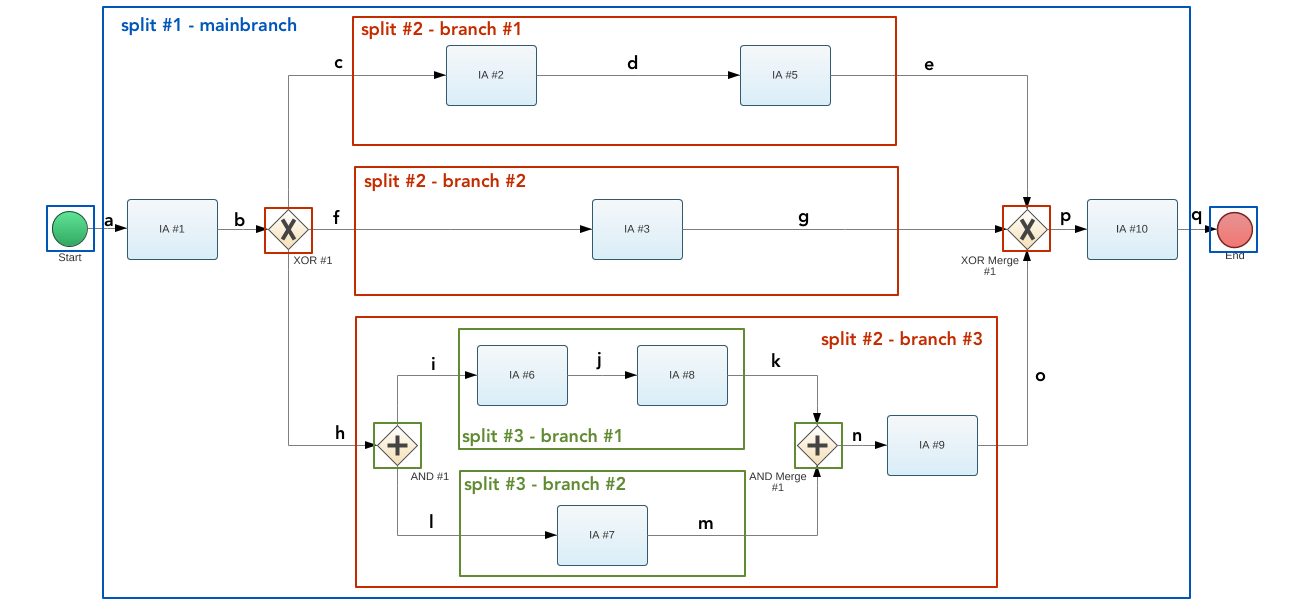
\includegraphics[width=0.9\textwidth]{src/images/graphTracking_1_edges.png}
\caption{Model Tracking Component - Concept}
\label{fig:graphTracking1}
\end{figure}

Figure \ref{fig:graphTracking1} illustrates the concept of this \textit{Model Tracking} component. In this example, there are in total three splits with the split nodes: start event (blue), exclusive gateway\#1 (red) and parallel gateway \#1 (green). The split with the start event as the split node and the end event as the merge node has always only one branch, the root branch. Technically, this is not a split in the sense of the terminology. But because of the underlying control flow logic and data model, which is shown in figure \ref{fig:graphTracking2}, that defines that every branch must be related to a split, this pseudo-split is necessary to keep track of the root branch.

\begin{figure}[htb]
\centering
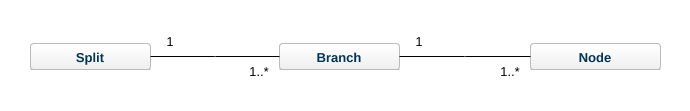
\includegraphics[width=0.8\textwidth]{src/images/graphtracking_dm.png}
\caption{Model Tracking Component - Data Model}
\label{fig:graphTracking2}
\end{figure}

The root branch (split \#1 - branch \#1) holds the set of ordered nodes: Interaction \#1, XOR gateway \#1, XOR merge \#1 and Interaction \#10. Split \#2 has three branches. The first branch contains the nodes Interaction \#2 and Interaction \#5. The second branch consists only of Interaction \#3 and the third branch contains AND gateway \#1, AND merge \#1 and Interaction \#9. At last, the third split consists of two branches, which hold the remaining interactions \#6, \#8 and \#7 respectively. Note that branches and therefore also splits, contain other splits, e.g. split \#2 contains split \#3 in branch \#3. This interleaving determines the hierarchy of the resulting RPST, which is shown in Figure \ref{fig:rpst_tree}. The root fragment is split \#1 and contains the non-trivial fragment \textit{split \#2} as well as the trivial fragments (edges) E = \{a, b, p, q\}. In turn \textit{split \#2} contains the non-trivial fragment \textit{split \#3} and the edges E = \{c, d, e, f, g, h, n, o\}. The last non-trivial fragment \textit{split \#3} contains the edges E = \{i, j, k, l, m\}.
\vspace{-0.25cm}
\begin{figure}[htb]
\centering
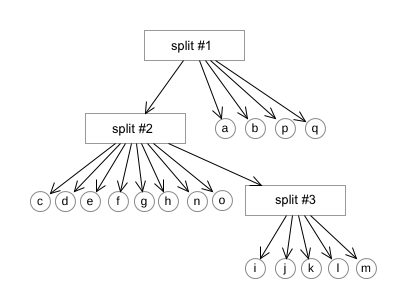
\includegraphics[width=0.6\linewidth]{src/images/graphTracking_rpst.png}
\caption{Refined Process Structure Tree}
\label{fig:rpst_tree}
\end{figure}

During the generation process, the current model build is maintained within the \textit{Model Tracking} component and simultaneously as a RPST graph. So far, there is no apparent necessity for the \textit{Model Tracking} component. But in order to automatically generate graphs representing choreography models, additional control flow logic is needed to ensure syntactically and behavioral correctness and to supervise the compliance with the build parameters. Therefor, each branch needs a status. This status indicates whether the branch is \textit{open}, \textit{splitted} or \textit{closed}. \textit{Open} defines, that the branch is not yet enclosed by the merge node of its corresponding split node and can further evolve by putting more nodes on its path. In turn, \textit{closed} defines that the branch is finalized and can not further evolve. Within the \textit{Model Tracking} component, a branch gets closed by putting the corresponding gateway merge node to the parent's branch and marking the branch as closed. Within the RPST graph, the merge node and an edge between the branch's last node with the merge node is added. A branch can also be in \textit{splitted} state, if it contains another split and none of this split's branches are yet closed, thus there exists no merge node for this split. In this case, a branch can not evolve until one of it's child split's branches is in state \textit{closed} and a merge node is placed on the branch. Then the state changes to \textit{open} again. For example, in figure \ref{fig:graphTracking3}, \textit{branch \#1} of \textit{split \#2} represents a branch in state \textit{split}, whereas the main branch is in state \textit{open} because \textit{branch \#2} of \textit{split \#1} is already closed by the merge node of \textit{split \#2}. When closing a branch, first it is necessary to determine if a branch is allowed to be closed, without violating the soundness of BPMN choreography models. This is dependent on the split node type of the branch. The premise is that if the split node type is a parallel gateway, the branch is determined as \textit{closable} only if there is an interaction on all its enclosed paths. This means, that if a branch has a child split, its not necessary that an interaction is on the parent branch itself but on the branches of its child split or even on a deeper nested branch.

\begin{figure}[htb]
\centering
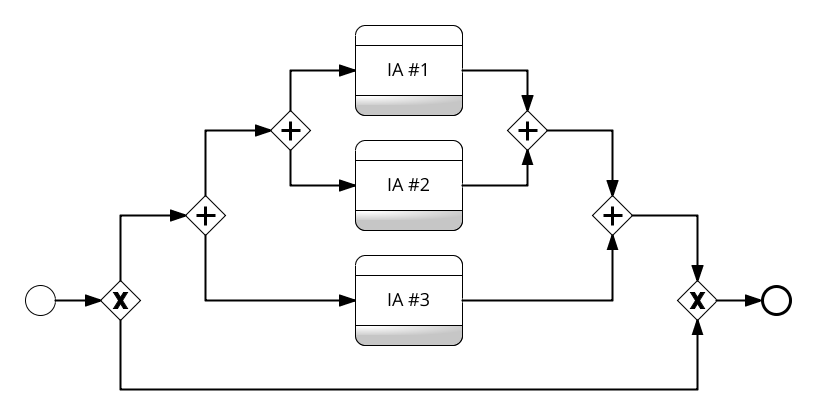
\includegraphics[width=0.7\textwidth]{src/images/choreo_min.png}
\caption{Minimum interactions reserved by remaining gateways}
\label{fig:graphTracking4}
\end{figure}
\vspace{-0.1cm}
For instance, see the upper branch of the second parallel gateway in Figure \ref{fig:graphTracking4}. The branch itself holds only another parallel gateway split node and a corresponding merge node but no interaction. This is valid because both branches of the parallel child split have an interaction and therefore also all enclosed paths of the parent branch. If the split node type is a exclusive gateway, it's allowed that one of the split's branches has no interaction on its path. For instance, see lowest branch of fist exclusive gateway in Figure \ref{fig:graphTracking4}. This depicts the circumstance that for an exclusive gateway, it's required to be able to also model a branch, where under certain process conditions no interaction between participants is necessary. This approach of tracking the status of the branches becomes crucial when only few remaining interactions are available and several branches are still open in the model. Because of the parametric limitation of the number of interactions, at a certain point in the build process or even directly in the beginning, if the proportion of specified gateways and interactions is small, interactions are not always allowed to be selected as next node type and not every open branch is allowed to be randomly selected for putting the next node into the model without resulting in a violation of the correctness of the model or exceeding the number of defined interactions. In order to determine whether this situation applies to a current point in a build process, the \textit{Model Tracking} component monitors the amount of \textit{free interactions} and \textit{reserved interactions}. 

Reserved interactions, are a subset of the remaining interaction that have either predetermined positions in the current graph (resInteractionsBranches) or will be needed in further paths created by not yet employed gateways (resInteractionsGateways). The exact amount of these reserved interactions depends on the number of non-closable branches of the current graph and the number of gateways that are not yet put into model. Regarding the current model, each open and non closable branch increases the amount of \textit{resInteractionsBranches} by one. Parallel gateways that are not yet placed into the graph will later create at least two new branches, which then again need at least one interaction on each of it's paths. Considering that a gateway node is allowed to be immediately followed by another gateways node without an interaction in between, the minimum amount of \textit{resInteractionsAndGateways} is \textit{remainingAndGateways} + 1. This premise also influences the impact of remaining exclusive gateways on the number of \textit{resInteractionsGateways}. Each remaining exclusive gateways only increases the number of \textit{resInteractionsGateways} by 1 if there is no more remaining parallel gateway. Because if there is also a remaining parallel gateway, the exclusive gateway could be put on a branch of the parallel gateway directly after the split and therefor the one needed interaction of the exclusive gateway is already considered in the calculation of \textit{resInteractionsAndGateways}. The influence of nested gateways onto the minimum amount of reserved interactions is illustrated in Figure \ref{fig:graphTracking4}. Given the parametric constraints \textit{numberOfInteractions = 3}, \textit{numberOfParallelGateways = 2} and \textit{numberOfExclusiveGateways = 1}, the figure represents one out of three possible resulting choreography models, which only differ in the sequence of used gateway types but not in the way of nesting and branching. After the amount of \textit{reserved interactions} is calculated, the number of \textit{free interactions} is determined by the difference between the amount of \textit{remaining interactions} and the number of \textit{reserved interactions}. Based on the values of the specified variables defined in Definition \ref{def:def1}, the node type of the next node to be put in the model and the corresponding position can be randomly selected without resulting in an incorrect model. For example, if the amount of \textit{free interactions} is $<$ 1, the random branch selection (position in the model) for putting the next node is limited to the branches that are not yet closable. On the other hand, if the amount of \textit{free interactions} $>$ 0, then all open branches can be selected for putting the next node. For the limitation of random branch selection, see also Algorithm \ref{alg:randBranch} and  Figure \ref{fig:graphTracking3}, which shows an unfinished choreography model at the point during the build process, assuming the parametric constrains numberOfInteractions = 6, numberOfAndGateways = 1 and numberOfExclusiveGateways = 1, where not all open branches are allowed to be selected for placing the node (in this case an interaction). In order to obtain a sound choreography model while not increasing the number of initially specified interactions, the sixth interaction is only allowed to be placed on branch \#2 of split \#3. In this scenario, \textit{reservedInteractionsTotal} equals one and \textit{freeInteractions} therefor equals zero. On the other hand, if assuming the total number of interactions being 7, all branches of split \#3 and the root branch are possible candidates for placing the sixth interaction, because at this point, \textit{freeInteractions} would equal one. In case of selecting the next possible node type, interactions are only allowed to be randomly selected, if the the amount of \textit{free interactions} $>$ 0 or not all remaining interactions are reserved by not yet consumed gateways.

\begin{Def}
	Let $x$ be the number of branches which are open and non-closable, \\$remainingInteractions$, all interactions not yet put into the model and \\$remainingXOR$ and $remainingAND$ the number of gateways not yet put into the model. Then
	\begin{center}
		\textbf{resInteractionsBranches} = x\\
		\textbf{resInteractionsAndGateways} = $remainingAND$ + 1\\
		\textbf{resInteractionsXORGateways} = \textbf{If} $remainingAND$ \textbf{$>$} 0 \textbf{Then} 0 \textbf{Else} 1\\
		\textbf{resInteractionsGateways} = $resInteractionsAndGateways$ + $resInteractionsXORGateways$\\
		\textbf{resInteractionsTotal} = $resInteractionsBranches$ + $resInteractionsGateways$\\
		\textbf{freeInteractions} = $remainingInteractions$ - $resInteractionsTotal$
	\end{center}
	\label{def:def1}
\end{Def}


\begin{figure}[]
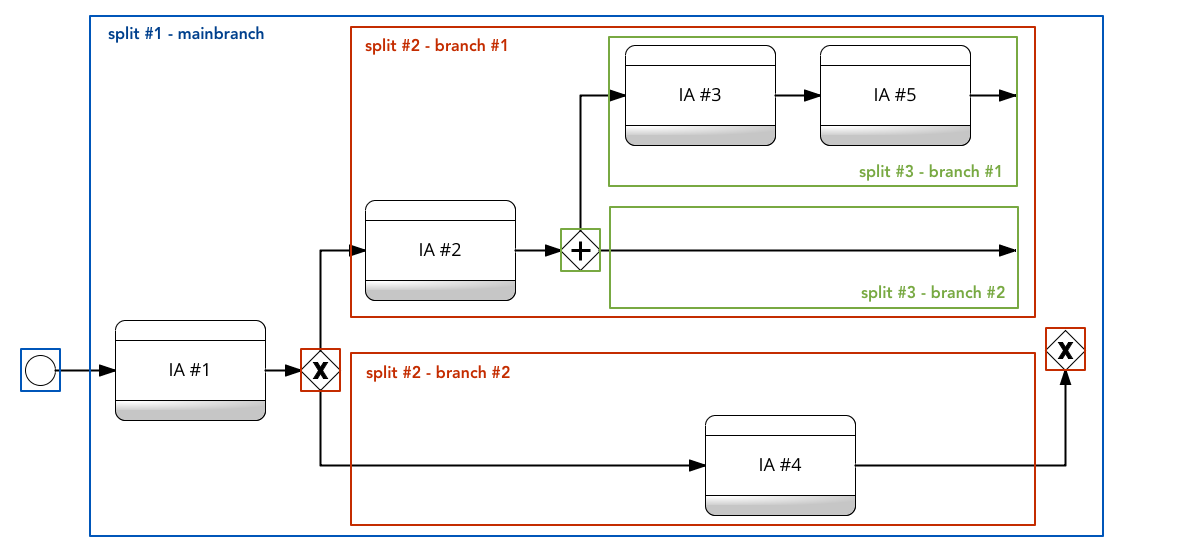
\includegraphics[width=1\textwidth]{src/images/choreo_branch_status.png}
\caption{Limitation of random branch selection}
\label{fig:graphTracking3}
\end{figure}
\vspace{-0.25cm}
The overall procedure of generating random choreography models is shown in Algorithm \ref{alg:choreoGen}. The input for a random model generation are the parametric constraints introduced in section \ref{sec:param_constraints}. At first, it is checked if the specified combination of the amount of interactions and gateways are sufficient for generating a sound model. This is the same evaluation as in determining the reserved interactions by remaining gateways. Therefore, the specified \textit{numberOfInteractions} must be greater or equal \textit{resInteractionsGateways}. If the validation is successful, the \textit{Model Tracking} component gets instantiated. Thereby, a split for the start event and the root branch is created. After this setup, the algorithm loops over the number of remaining interactions until all interactions are put into the model. Within each loop, at first a node type for the next node is randomly selected out of the pool of remaining nodes. This can be an interaction, exclusive or parallel gateway, depending on the number of free and reserved interactions as already explained. The algorithm for random possible node type selection is shown in Algorithm \ref{alg:randNodeType}.\\

\begin{algorithm}[H]
\small
\DontPrintSemicolon
\SetAlgoLined
\Begin{
	possibleNodeTypes $\leftarrow$ \{\}\;
	\If{freeInteractions $>$ 0 $\lor$ remainingInteractions > resInteractionsGateways}{
		possibleNodeTypes $\leftarrow$ possibleNodeTypes $\cup$ Interaction\;
	}
	\If{remainingParallelGateways $>$ 0}{
		possibleNodeTypes $\leftarrow$ possibleNodeTypes $\cup$ ParallelGateways\;
	}
	\If{remainingExclusiveGateways $>$ 0}{
		possibleNodeTypes $\leftarrow$ possibleNodeTypes $\cup$ ExclusiveGateways\;
	}
	\Return random NodeType of possibleNodeTypes\;	
}
\caption{getRandomNodeType()}
\label{alg:randNodeType}
\end{algorithm}
\vspace{0.4cm}
After a node type has been randomly selected, a position in the model is determined for placing a node of the previously selected node type by randomly selecting a possible open branch. Which branches are in the pool of possible, selectable branches, is again depending on whether there are free interactions available or not. If there are free interactions left, all open branches are allowed to be selected, independent of the priorly selected node type. Otherwise, only branches that are not closable are allowed to be included in the pool of possible branches. The algorithm for random possible branch selection is shown in Algorithm \ref{alg:randBranch}.\\

\begin{algorithm}[H]
\small
\DontPrintSemicolon
\SetAlgoLined
\Begin{
	possibleBranches $\leftarrow$ \{\}\;
	\eIf{freeInteractions $>$ 0 }{
		possibleBranches $\leftarrow$ all open branches\;
	}{
		possibleBranches $\leftarrow$ all not closable branches\;
	}
	\Return random Branch of possibleBranches\;	
}
\caption{getRandomBranch()}
\label{alg:randBranch}
\end{algorithm}
\vspace{0.4cm}
In the next step, the randomly selected branch is checked whether it's closable or not and if so gets closed by random. This doesn't apply to the root branch to make sure that there is always one branch where the model can further evolve. This step of random branch closing is necessary to obtain balanced choreography models regarding nested branches. If there would be no random branch closing mechanism, the resulting models would be very similar. A mechanism that closes branches whenever they are possible to close would only result in models with lesser nested branches whereas a mechanism that never closes branches would result in models that have highly nested branching. If the selected branch gets randomly closed, a merge node for the selected branch's split is created and added to the parent branch. Additionally, in the data model of the corresponding split, the merge node gets noted in order to assure that the last nodes of the other branches of this split will get connected with the same merge node as soon as they get closed. Finally, the algorithm jumps back to the beginning of the loop and starts again with randomly selecting a possible node type for the next node to be placed in the model.\\

\begin{algorithm}[H]
\small
\DontPrintSemicolon
\SetAlgoLined
\SetKwInOut{Input}{Input}\SetKwInOut{Output}{Output}
\Input{ 
\begin{itemize}[label={--}]
\setlength\itemsep{0em}
\item $minBranching \leftarrow$ 2\;
\item $maxBranching \leftarrow$ user specified upper branch amount border\;
\item $freeInteractions \leftarrow$ number of currently free interactions
\end{itemize}
}
\Begin{
	\eIf{freeInteractions $\geq$ 0}{
		$currentMaxBranching \leftarrow minBranching + freeInteractions$\;
		\If{currentMaxBranching $>$ maxBranching}{
			$currentMaxBranching \leftarrow maxBranching$\;
		}
	}{
		$currentMaxBranching \leftarrow minBranching$\;
	}
	
	\Return random value between $minBranching$ and $currentMaxBranching$\;	
}
\caption{getRandomBranchAmount()}
\label{alg:randBranchAmount}
\end{algorithm}
\vspace{0.5cm}
By the time a branch is not randomly closed, a node of the predefined node type gets instantiated. In case of an interaction, only the plain object without any sender, receiver or message gets instantiated. Is the selected node type a gateway, the number of branches is determined by randomly selecting a number between 2 and the current maximum branching amount. The maximum branching amount is generally limited by the user specified max branching parameter. But again, due to the limitation of interactions, the specified maximum amount of branches can not be adducted as the upper border without considering the current amount of free interactions. If only the user specified upper branching border (max. branching parameter) is adducted, there is a high chance that this would result in an inconsistent model, because the remaining interactions are insufficient for all paths created. In order to prevent this, the possible upper limit is determined dynamically each time a gateway node is put into the model by taking the minimum branching amount, which is always two, and adding the amount of free interactions. The algorithm for random possible branch amount selection is shown in Algorithm \ref{alg:randBranchAmount}. After a random number of branches is determined, the gateway node is added to the assigned branch and the corresponding split and branches are instantiated within \textit{Model Tracking}. Finally, the amount of the selected node type is decreased by one and the newly created edge between the preceding and the new node gets added into the RPST graph, before the loop starts over by selecting a random node type for the next node to be put into the model.\\

\begin{algorithm}[H]
\small
\DontPrintSemicolon
\SetAlgoLined
\SetKwInOut{Input}{Input}\SetKwInOut{Output}{Output}
\Input{ 
\begin{itemize}[label={--}]
\setlength\itemsep{0em}
\item $mainSplit \leftarrow$ split of root branch\;
\end{itemize}
}
\SetKwProg{Fn}{Function}{}{}
\Begin{
	\ForEach{branch of split.branches}{
		\ForEach{node of branch.nodes}{
			\If{node is gateway}{
				$closeSplit(split)$\;
			}
		}
		\If{branch is open}{
			$branch.close()$\;
		}
	}
}
\Fn{branch.close()}{
	$split \leftarrow$ split of branch\;
	\eIf{split.mergeNode == null}{
		$mergeNode \leftarrow$ instantiate merge node of gateway type\;
		$split.mergeNode \leftarrow$ mergeNode\;
		$branch.state \leftarrow$ closed\;
	}{
		$branch.state \leftarrow$ closed\;
	}
}
\caption{closeSplit(Split)}
\label{alg:finishModel}
\end{algorithm}
\vspace{0.5cm}
After all interactions and gateways are put into the model, the loop ends and all still open branches are getting closed. Algorithm \ref{alg:finishModel} displays the function to close all yet open branches by looping the model recursively. At this point, where the model doesn't further evolve, a branch is closed if the belonging split has a merge node assigned. If this is not the case, a merge node is created, added to the corresponding branch and assigned to the split.\\

\begin{algorithm}{hbt}
\small
\DontPrintSemicolon
\SetAlgoLined
\SetKwInOut{Input}{Input}\SetKwInOut{Output}{Output}
\Input{ 
\begin{itemize}[label={--}]
\setlength\itemsep{0em}
\item $remainingNodes \leftarrow$ number of nodes by type
\item $participants \leftarrow$ number of participants
\item $loops \leftarrow$ number of loops
\item $graph \leftarrow$ RPST graph
\end{itemize}
}
\SetKwProg{Fn}{Function}{}{}
\SetKw{Continue}{continue}
\Begin{
	\If{number of interactions $\leq$ number of gateways + 1}{
		model generation not possible\;
	}
	$modelTracking \leftarrow$ initialize model tracking component\;
	\While{$remainingInteractions > 0$}{ 
		$nextNodeType \leftarrow$ getRandomNodeType()\;
		$selectedBranch \leftarrow$ getRandomBranch()\;
		$precedingNode \leftarrow$ last node of $selectedBranch$\;
		\If{$precedingNode$ is $NULL$}{
			$precedingNode \leftarrow$ split node of $selectedBranch$\;
		}
		\eIf{$selectedBranch$ is closable}{
			close branch by random\;
			\If{closed}{
				\Continue
			}
		}{
			$nextNode \leftarrow$ instantiate node of $nextNodeType$\;
			\If{$nextNodeType$ is Gateway}{
				$branchCount \leftarrow$ getRandomBranchCount()\;
				$split \leftarrow$ instantiate new split\;
				$modelTracking.splits \leftarrow$ split\; 
				\For{$i \leftarrow$ 0 $branchCount$}{
					$branch \leftarrow$ instantiate new branch\;
					$split.branches \leftarrow branch$\;
					$i \leftarrow i$ + 1\;
				}
			}
			$selectedBranch.nodes \leftarrow$ $selectedBranch.nodes \cup nextNode$\;
			decrease $remainingNodes$ of $nextNodeType$\;
			add edge between $precedingNode$ and $nextNode$ to $graph$\;
		}
	}
	close still open splits\;
	add end event to root branch\;
	enrich interactions with reasonable sender and receiver sequence\;
}
\caption{Generate Choreography Model}
\label{alg:choreoGen}
\end{algorithm}

At this point the generated model is already syntactically correct because all model elements are used and connected according to BPMN specification. To achieve also behavioral correctness in choreography models, beside a correct sequence flow, a message flow must be incorporated. Therefore, a sender and receiver must be assigned to each interaction in order to form a valid sender-receiver sequence. Thereby, the sender of a succeeding interaction Q must always be either the sender or receiver of the directly preceding interaction P on the path. If this rule is not considered and the sender of a directly succeeding interaction Q is neither the sending nor the receiving participant of the directly preceding interaction P, a flawless execution of the process is not possible, because the sender of interaction Q will never know if the directly preceding interaction P has been performed yet. In case of gateways, additionally it is ensured that the receiver of the last interaction of each branch of the gateway is the same in order to determine a possible common sender for the succeeding interaction after the merge. Figure \ref{fig:messageFlow} illustrates a correct message flow within choreography models.  

\begin{figure}[htp]
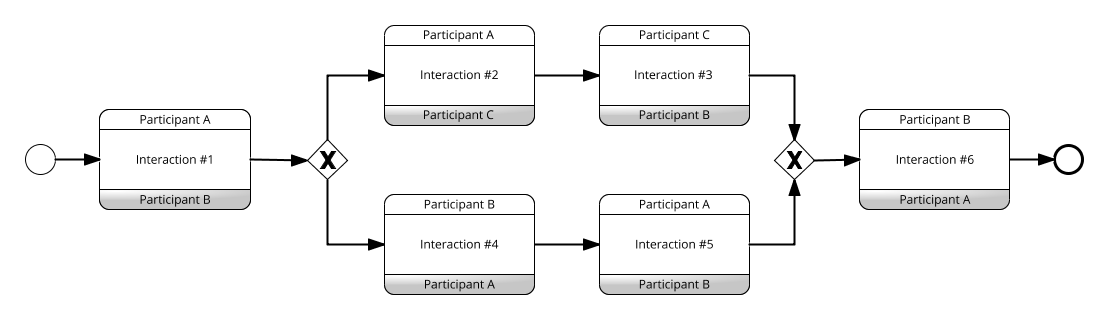
\includegraphics[width=1\textwidth]{src/images/messageFlow.png}
\caption{Message Flow - Sender/Receiver sequence}
\label{fig:messageFlow}
\end{figure}

Note that because of the fact that the sequence flow is first build without considering the corresponding message flow, it is likely that at some points an additional interaction must be inserted into the model to satisfy the above stated rules of sender-receiver sequences.

\subsection{Compliance Rules Assignment}
As pointed out in Chapter \ref{sec:overallprocesscontroller}, first a model is generated and afterwards it is checked whether the interaction sequence specified within the compliance rules can be applied to the generated model. Instead of considering the imposed compliance rule during the choreography generating, the followed approach was favored to allow users to specify compliance rules, which then can be imposed to also already existing choreography models in order to check if this particular model complies to the specified rules. Until now, the generated model complies only to the parametric constraints. The logic of specifying and imposing compliance rules is implemented within the \textit{Compliance Controller} component.\\

When specifying compliance rules to which the choreography model must comply, it must be checked whether the imposed rules are consistent with one another. In the context of the four supported patterns (see Table \ref{tab:compl_patterns}), this applies only to the two order patterns (LeadsTo and Precedes). For instance, consider the following set of compliance rules:

\begin{itemize}
\item \textit{CR-1}: P LeadsTo Q
\item \textit{CR-2}: Q LeadsTo S
\item \textit{CR-3}: S Precedes P
\end{itemize}

In this example, the rule \textit{CR-1} in combination with \textit{CR-2} is in conflict with \textit{CR-3}, because \textit{CR-1} and \textit{CR-2} determine, that the involved activities must occur in the order P-Q-S, whereas \textit{CR-3} constrains, that activity S must occur before activity P, which is in violation of the order determined by \textit{CR-1} and \textit{CR-2}. Algorithm \ref{alg:conflictCheck} shows the conflict checking procedure implemented within the \textit{Compliance Controller}. \\

\begin{algorithm}[H]
\small
\DontPrintSemicolon
\SetAlgoLined
\SetKwInOut{Input}{Input}
\SetKwInOut{Output}{Output}
\Input{ 
\begin{itemize}[label={--}]
\item compliance rule $cr$
\item dictionary $orderDependencies$ consisting of Interactions $P$ and their succeeding Interactions $S$
\end{itemize}
}
\SetKwProg{Fn}{Function}{}{}
\Begin{
	\If{$cr$ is order pattern}{
		$p \leftarrow$ preceding interaction of $cr$\;
		$s \leftarrow$ succeeding interaction of $cr$\;
		\eIf{!orderConflictCheck($p, s$)}{
			add $cr$ to $complianceRules$\;
			\eIf{$p \in P$ of $orderDependencies$}{
				add $s$ to succeeding interactions $S$ of $p$
			}{
				add $p$ to $orderDependencies$\;
				add $s$ to succeeding interactions $S$ of $p$ 
			}	
		}{
			add $cr$ to $conflictedRules$\;
		}
	}	
}
\Fn{orderConflictCheck($p, s$)}{
	\eIf{$s \in P$ of $orderDependencies$}{
		\ForEach{$s \in S$ of $p$}{
			\uIf{$s$ == $p$}{
				\Return \textbf{true}
			}\uElseIf{orderConflictCheck($s, p$)}{
				\Return \textbf{true}
			}
		}
	}{
		\Return \textbf{false} 	
	}
}
\caption{Adding Compliance Rules}
\label{alg:conflictCheck}
\end{algorithm}
\vspace{0.5cm}
The result of this procedure is a set of conflict free compliance rules, which determines a specific order sequence between the involved interactions. The specific interactions of the compliance rules are then eventually assigned to the existing interactions within the before generated model in a way that it complies to the interaction order and the compliance rules. Therefore, the first step is to determine all possible positions within the model for each compliance rule. The result is a set of possible position combinations (interactions placed in the model during initial choreography generation) for the compliance rule specified Interaction P and Interaction Q. For each possible position of Interaction P there has to be at least one possible position for Interaction Q. The rules that determine applicable positions for the four implemented compliance patterns are shown in Definitions \ref{def:leadsto} - \ref{def:exists}. \\

The difference between the determination of possible positions for the patterns \textit{LeadsTo} and \textit{Precedes} is that in case of \textit{P LeadsTo Q} the position for Interaction Q must always be reached after the position of Interaction P has been reached, whereas in case of \textit{P Precedes Q} the Interaction Q must only be possible to reach afterwards. In other words, if Interaction Q is executed, Interaction P must have occurred before. This means that unlike for the \textit{LeadsTo} pattern, in case of a \textit{Precedes} the succeeding interaction Q can also be inside an exclusive branch of the subsequent path of interaction P. For example, let P be assigned to \textit{Interaction IA 2} of the choreography model shown in figure \ref{fig:crassign}. In case of a \textit{Precedes} pattern, the set of possible interactions for Q is \textit{Q}\textsubscript{IA2} = \{IA 3, IA 4, IA 5, IA 6, IA 7, IA 8, IA 9, IA 10, IA 11, IA 12, IA 13, IA 14\}. These are all interactions that are possibly reachable after IA 2 has been reached. On the other hand, in case of \textit{LeadsTo}, the set of possible interaction assignments \textit{Q}\textsubscript{IA2} only includes \{IA 13, IA 14\}, because if IA 2 has been reached, only these two are always possible to be reached afterwards. Additionally to this rules, for a given P assigned within a parallel branch, the succeeding interaction Q is not allowed to be assigned to a position of another parallel branch, because there is no control mechanism that ensures the correct sequence of parallel interactions. This must be considered for both order patterns.

\begin{Def}
	Possible position assignments for the interactions P and Q of a compliance pattern P LeadsTo Q are as following:
	\begin{center}
		\textbf{Interaction P} = An interaction that has interactions on its subsequent paths that will always be reached.\\
		\textbf{Interaction Q} = An interaction that will always be reached after Interaction P has been reached.\\
	\end{center}
	\label{def:leadsto}
\end{Def}

\begin{Def}
	Possible position assignments for the interactions P and Q of a compliance pattern P Precedes Q are as following:
	\begin{center}
		\textbf{Interaction P} = An interaction that is always reached prior to Interaction Q.\\
		\textbf{Interaction Q} = An interaction that has interactions on its preceding path that were always reached prior to Interaction Q.\\
	\end{center}
	\label{def:precedes}
\end{Def}

The two occurrence patterns \textit{Universal} and \textit{Exists} differ only in that in for \textit{P Universal}, the position of interaction P must always be reached throughout process execution, whereas for \textit{P Exists} the position of interaction must only be reachable or in other words must be defined within the model.

\begin{Def}
	Possible position assignments for the interaction P of a compliance pattern P Universal are as following:
	\begin{center}
		\textbf{Interaction P} = An interaction that will always be reached.\\
	\end{center}
	\label{def:universal}
\end{Def}

\begin{Def}
	Possible position assignments for the interaction P of a compliance pattern P Exists are as following:
	\begin{center}
		\textbf{Interaction P} = An interaction that can be reached.\\
	\end{center}
	\label{def:exists}
\end{Def}

\begin{figure}[H]
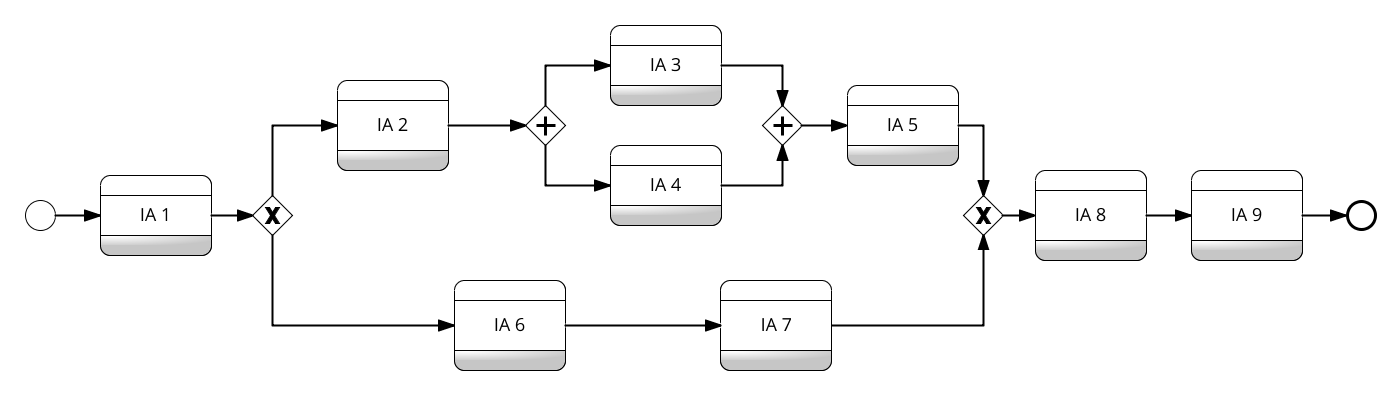
\includegraphics[width=1\textwidth]{src/images/cr_assign.png}
\caption{Compliance Rule Assignment}
\label{fig:crassign}
\end{figure}

If the interactions used for specifying the rules are disjoint between all the compliance rules, the sets of assignment combinations are already sufficient to assign the involved interactions to positions that result in a model that is compliant with the opposed rules. But if there are particular interactions that are used in more than one compliance rule specification, the intersection of the interaction's possible assignments of all involved compliance rules represents the set of possible assignments for this particular interaction. For example, consider the choreography model shown in Figure \ref{fig:crassign} and the following compliance rules within which interaction B and C are each specified in the compliance rules \textit{CR-1} and \textit{CR-2}:

\begin{itemize}
\item \textit{CR-1}: Interaction A LeadsTo Interaction B
\item \textit{CR-2}: Interaction C Precedes Interaction B
\item \textit{CR-3}: Universal Interaction C
\end{itemize}

The three compliance rules form two valid order sequences between the three specified interactions: Interaction A $\rightarrow$ Interaction C $\rightarrow$ Interaction B and Interaction C $\rightarrow$ Interaction A $\rightarrow$ Interaction B. More than one valid order indicates that there is no strict sequence between some defined interactions. For example, within the three stated compliance rules there is no determined sequence between \textit{Interaction A} and \textit{Interaction C}. Thus, that in this case, the two interactions can be also assigned to paths that are parallel to one another. If there is more than one possible order, the implemented procedure choses one by random.

\begin{algorithm}[hbt]
\small
\DontPrintSemicolon
\SetAlgoLined
\SetKwInOut{Input}{Input}\SetKwInOut{Output}{Output}
\Input{
	$interactionOrder \leftarrow$ ordered CR interactions\;
} 
\SetKwProg{Fn}{Function}{}{}
\SetKw{Continue}{continue}
\Begin{
	determinePossibleAssignments()\;
	\ForEach{interaction in interactionOrder}{
		\If{!assignInteraction(interaction)}{
			\Return \textbf{false}\;
		}
	}
}
\Fn{assignInteraction(Interaction ia)}{
	$affectedCRs \leftarrow$ all compliance rules with ia involved\;
	$crPossibleAssignments \leftarrow$ HashMap$<$cr, model interactions$>$\;
	$modelAssignments \leftarrow$ HashMap$<$cr interaction, model interaction$>$\;  
	\ForEach{cr in affectedCRs}{
		\uIf{ia is specified P of cr}{
			$crPossibleAssignments \leftarrow$ add all possible model interactions for P\;  
		}\uElseIf{ia is specified Q of cr}{
			$pAssignment \leftarrow$ already assigned model interaction of P
			$crPossibleAssignments \leftarrow$ add all possible model interactions of Q for the given P\; 
		}
	}
	$commonPossibleAssignments \leftarrow$ common model interactions between all crPossibleAssignment entires\;
	\eIf{commonPossibleAssignments is not empty}{
		$selectedInteraction \leftarrow$ get interaction with most succeeding interactions out of commonPossibleAssignments\;
		$modelAssignments \leftarrow$ add ia with selected model interaction\;
		\Return \textbf{true}\;
	}{
		\Return \textbf{false}\;
	}
}
\caption{Compliance Rules Assignment}
\label{alg:imposecr}
\end{algorithm}

After the interaction order is set, for every specified compliance rule the possible model positions are determined independently, based on the rules defined in Definitions \ref{def:leadsto} to \ref{def:exists}.  The result of this step is shown in Tables \ref{tbl:crAssignment1} to \ref{tbl:crAssignment3}. These two steps are the preconditions for the actual assignment of the interactions into the existing model, which is shown in Algorithm \ref{alg:imposecr}. The assignment procedure iterates over the interaction order and for each interaction the intersection of the possible assignments of all affected compliance rules (commonPossibleAssignments) is calculated. Is the current interaction specified as the succeeding interaction of an affected order compliance rule, the possible model positions of this rule are limited to the succeeding model positions of the corresponding, already assigned, preceding interaction. For instance, let the order of the example compliance rules be C $\rightarrow$ A $\rightarrow$ B and let \textit{Interaction C} be already assigned to \textit{IA 1} and \textit{Interaction A} to \textit{IA 3} of the model shown in Figure \ref{fig:crassign}. In order to determine the possible model positions for \textit{Interaction B}, the intersection of the sets of possible positions for \textit{Interaction B} of the affected rules \textit{CR-1} and \textit{CR-2} has to be determined: 

\begin{itemize}
\item \textit{CR-1}: \{IA5, IA8, IA9\}
\item \textit{CR-2}: \{IA2, IA3, IA4, IA5, IA6, IA7, IA8, IA9\}
\item \textit{CR-1 $\cap$ CR-2}: \{IA5, IA8, IA9\}
\end{itemize}

Is the resulting intersection of the sets of possible assignments empty, then there is no valid position in the model where the interaction could be assigned to. In this case, the whole assignment process fails and results in a failed choreography build process, which triggers a new build process from the beginning (see Algorithm \ref{alg:choreographyController} - line 6). Is the intersection of possible model positions not empty, the procedure choses the interaction that has the most interactions on it's succeeding path, or in terms of RPST, the highest ranked trivial fragment on the hierarchy. This ensures, that the assignment process does not fail because of higher ranked interactions being assigned to positions at the end of the model, so that there are no valid positions left for lower ranked ones.  

\begin{table}[H]
\centering
\begin{tabular}{ll}
\multicolumn{1}{l|}{Interaction A}    & Interaction B                \\ \hline
\multicolumn{1}{l|}{IA1}  & \{IA8, IA9\}                      \\
\multicolumn{1}{l|}{IA2}  & \{IA3, IA4, IA5, IA8, IA9\}                           \\
\multicolumn{1}{l|}{IA3}  & \{IA5, IA8, IA9\} \\
\multicolumn{1}{l|}{IA4}  & \{IA5, IA8, IA9\}          \\
\multicolumn{1}{l|}{IA5}  & \{IA8, IA9\}                \\
\multicolumn{1}{l|}{IA6}  & \{IA7, IA8, IA9\}                 						\\
\multicolumn{1}{l|}{IA7}  & \{IA8, IA9\}                \\
\multicolumn{1}{l|}{IA8}  & \{IA9\}                     \\
\multicolumn{1}{l|}{IA9}  & \{\}               \\ \hline
\end{tabular}
\caption{Possible assignment combinations for CR-1}
\label{tbl:crAssignment1}
\end{table}

\begin{table}[H]
\centering
\begin{tabular}{ll}
\multicolumn{1}{l|}{Interaction C}    & Interaction B                \\ \hline
\multicolumn{1}{l|}{IA1}  & \{IA2, IA3, IA4, IA5, IA6, IA7, IA8, IA9\}                      \\
\multicolumn{1}{l|}{IA2}  & \{IA3, IA4, IA5\}                           \\
\multicolumn{1}{l|}{IA3}  & \{IA5\} \\
\multicolumn{1}{l|}{IA4}  & \{IA5\}          \\
\multicolumn{1}{l|}{IA5}  & \{\}                \\
\multicolumn{1}{l|}{IA6}  & \{IA7\}                     \\
\multicolumn{1}{l|}{IA7}  & \{\}                \\
\multicolumn{1}{l|}{IA8}  & \{IA9\}                     \\
\multicolumn{1}{l|}{IA9}  & \{\}               \\ \hline
\end{tabular}
\caption{Possible assignment combinations for CR-2}
\label{tbl:crAssignment2}
\end{table}


\begin{table}[H]
\centering
\begin{tabular}{l}
Interaction C \\ \hline
IA1 \\
IA8 \\
IA9 \\ \hline
\end{tabular}
\caption{Possible assignments for CR-3}
\label{tbl:crAssignment3}
\end{table}

\subsection{Deriving the Collaboration Models}

Following the introduced \textit{top-down approach}, the collaboration model as well as the public and private models of each partner are derived from the generated choreography model. As already mentioned, the public models are projections of the choreography model, which means that they represent the view on the collaboration process from the perspective of each involved participant, while focusing on the process of one participant at a time. They only include activities that are necessary to communicate with other process participants. The private models are then enhanced versions of the public models. Additionally, they include internal process activities that don't involve interaction with other participants and that are not relevant for other participants to know. At last, the collaboration model is the interconnection between the public models of each participant. Together they form a holistic view on the whole collaboration process and is therefore a different representation of the choreography model, without any information loss.\\
In the process of deriving the models, each interaction of the choreography model results in a send and receive task in the corresponding public models of the involved partners. In the public model of the initiating participant of an interaction, a send task is inserted and in the model of the receiving participant a corresponding receive task. Additionally, for each public model, it is tried to reduce the model's sequence flow as much as possible without violating the underlying, predetermined sequence flow of the choreography model. Thereby, each gateway of the choreography model is checked for interactions within its subsequent paths involving the current participant. If there are none, the gateway and it's subsequent paths are not put into the public model of this participant.\\  

\begin{figure}[H]
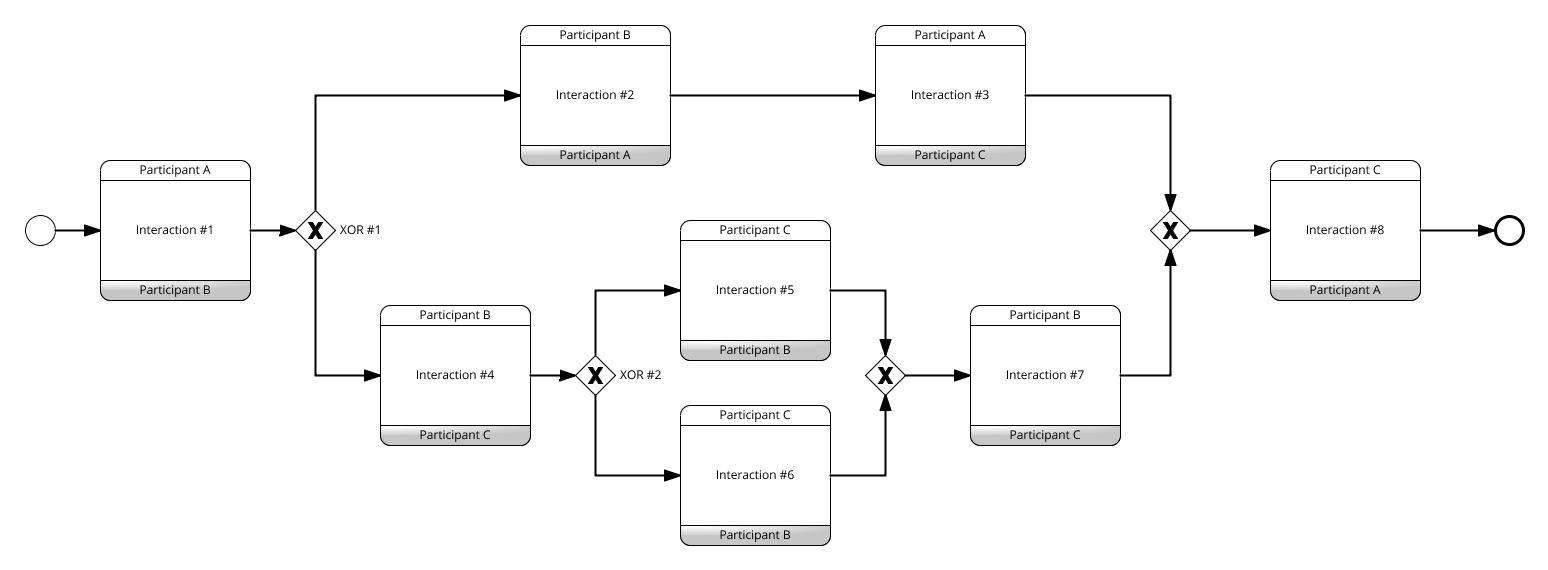
\includegraphics[width=1\textwidth]{src/images/choreo2public_choreo.png}
\caption{Choreography Model}
\label{fig:choreo2public}
\end{figure}

For instance, the choreography model shown in figure \ref{fig:choreo2public} would result in the three public models shown in Figures \ref{fig:choreo2public_pub} to \ref{fig:choreo2public_pub3}. The public model of Participant A (figure \ref{fig:choreo2public_pub}) is the only model where the sequence flow can be reduced in comparison to the choreography model. Because the lower path of the exclusive gateway \textit{XOR \#1} does not involve interactions that affect participant A, the whole path with all it's subsequent paths are not necessary and therefor not put into the public model.\\

\begin{figure}[H]
\centering
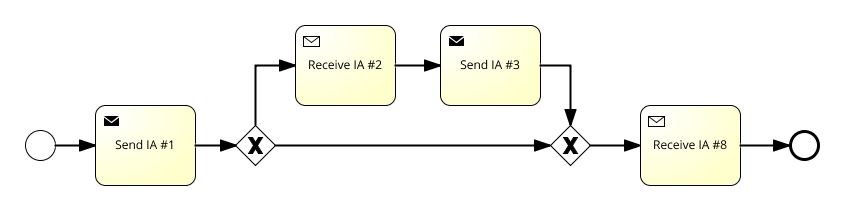
\includegraphics[width=0.8\textwidth]{src/images/choreo2public_pub1.png}
\caption{Public Model - Participant A}
\label{fig:choreo2public_pub}
\end{figure}

\begin{figure}[H]
\centering
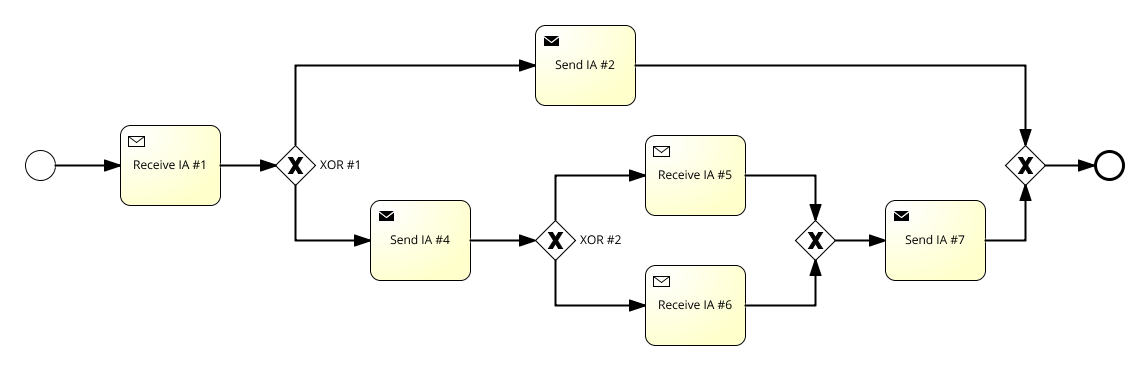
\includegraphics[width=0.8\textwidth]{src/images/choreo2public_pub2.png}
\caption{Public Model - Participant B}
\label{fig:choreo2public_pub2}
\end{figure}

\begin{figure}[H]
\centering
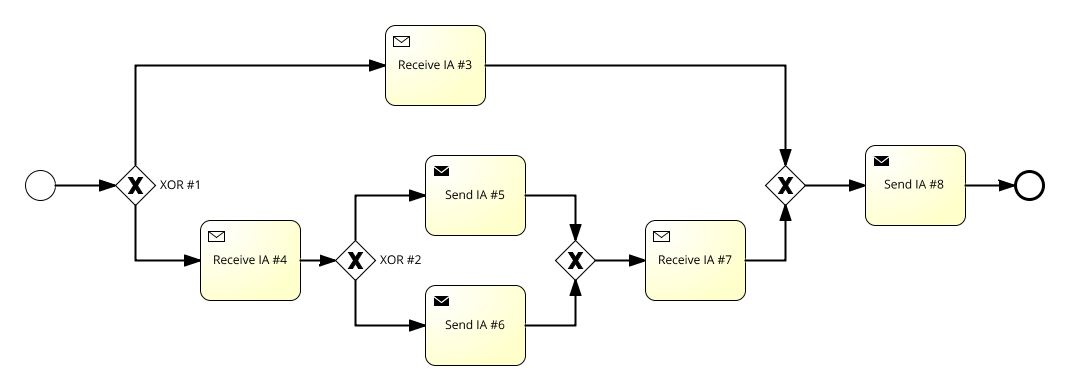
\includegraphics[width=0.8\textwidth]{src/images/choreo2public_pub3.png}
\caption{Public Model - Participant C}
\label{fig:choreo2public_pub3}
\end{figure}

In order to derive the private models from the public models, the public models are randomly enriched with private tasks, as well as some additional sequence flow elements (gateways) without violating the predefined sequence flow. The public models could also be used as private models without the enrichment, but because in real process scenarios, it is not likely that a participant does only perform public, interacting tasks, this enrichment is implemented. Figure \ref{fig:choreo2public_pr1} shows a possible outcome of a private model for participant A. 

\begin{figure}[H]
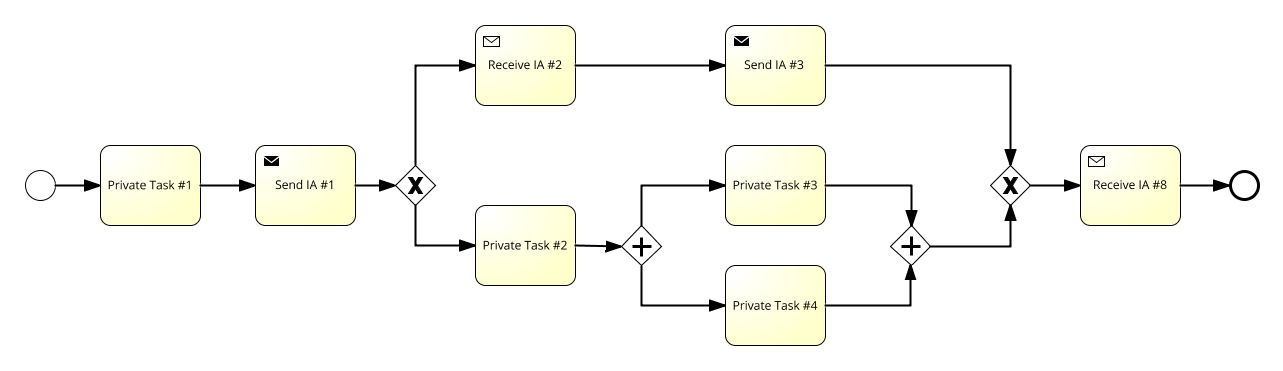
\includegraphics[width=1\textwidth]{src/images/choreo2public_pr1.png}
\caption{Possible Private Model - Participant A}
\label{fig:choreo2public_pr1}
\end{figure}

\section{Model Translation to BPMN/XML} \label{sec:bpmntranslation}
BPMN is the standard for describing business processes of any kind and therefore it is necessary to translate the generated process collaboration models in order to make them shareable and usable by a broad audience. Also, if some conventions are respected, the translated private models are out of the box executable and therefore the process can be tested by typical process engines. In order to translate the RPST representation of the models to BPMN/XML, the internal model elements for events, tasks, gateways, edges and participants must be mapped to the corresponding BPMN elements (see Table \ref{tab:flow_objects}) of the different model types and a process for generating a valid BPMN file must be designed. It has to be mentioned that the resulting BPMN/XML files only contain the formal process description. A generation of a the graphical process description will not take place. The following Table \ref{tbl:common2bpmn} shows the mapping of model type independent objects. These objects are used in all different model types and are therefore also common in the different BPMN models. Each model object is referenced by or has a reference to one or more other objects. For instance, the edges between flow objects do always refer to the flow objects (tasks and gateways) that are connected through this edge or, in case of an interaction, the message being sent is referenced. For this purpose, each model object has a unique id that also must be generated during the translation process.\\

\lstset{language=XML, morekeywords={definitions, encoding, xmlns, typeLanguage, targetNamespace, xsi:schemaLocation, message, id, name, choreography, isClosed, participant, messageFlow, messageRef, sourceRef, targetRef, choreographyTask, initiatingParticipantRef, incoming, outgoing, participantRef, messageFlowRef, startEvent, endEvent, parallelGateway, exclusiveGateway, gatewayDirection, sequenceFlow, sendTask, receiveTask, task}, basicstyle=\tiny, breaklines=true}

\begin{table}[H]
\centering
\begin{tabular}{l|l}
\multicolumn{1}{c|}{\textbf{Internal Object}} & \multicolumn{1}{l}{\textbf{BPMN/XML Element}}     \\ \hline
Participant &
\begin{lstlisting}
<participant id="(unique-id)" name="(name)"/>       
\end{lstlisting}\\ \hline
Start Event &
\begin{lstlisting}
<startEvent id="(unique-id)" name="">
  <outgoing>ref-to-sequenceFlow</outgoing>
</startEvent>       
\end{lstlisting} \\ \hline
End Event &
\begin{lstlisting}
<endEvent id="(unique-id)" name="">
  <incoming>ref-to-sequenceFlow</incoming>
</startEvent>       
\end{lstlisting} \\ \hline
Parallel Gateway &
\begin{lstlisting}
<parallelGateway id="(unique-id)" name="" 
  gatewayDirection="Diverging">
      <incoming>ref-to-sequenceFlow</incoming>
      <outgoing>ref-to-sequenceFlow</outgoing>
      <outgoing>ref-to-sequenceFlow</outgoing>
</parallelGateway>

<parallelGateway id="(unique-id)" name="" 
  gatewayDirection="Converging">
      <incoming>ref-to-sequenceFlow</incoming>
      <incoming>ref-to-sequenceFlow</incoming>
      <outgoing>ref-to-sequenceFlow</outgoing>
</parallelGateway>      
\end{lstlisting} \\ \hline
Exclusive Gateway &
\begin{lstlisting}
<exclusiveGateway id="(unique-id)" name="" 
  gatewayDirection="Diverging">
      <incoming>ref-to-sequenceFlow</incoming>
      <outgoing>ref-to-sequenceFlow</outgoing>
      <outgoing>ref-to-sequenceFlow</outgoing>
</exclusiveGateway>

<exclusiveGateway id="(unique-id)" name="" 
  gatewayDirection="Converging">
      <incoming>ref-to-sequenceFlow</incoming>
      <outgoing>ref-to-sequenceFlow</outgoing>
      <outgoing>ref-to-sequenceFlow</outgoing>
</exclusiveGateway>       
\end{lstlisting} \\ \hline
Edge & 
\begin{lstlisting}
<sequenceFlow id="(unique-id)" name="" 
  sourceRef="(ref-to-flow-object)" 
    targetRef="(ref-to-flow-object)"/>          
\end{lstlisting} \\ \hline
Message & 
\begin{lstlisting}
<message id="(unique-id)" name=""/>

<messageFlow id="(unique-id)" messageRef="(ref-to-message)" 
	sourceRef="(ref-to-sendTask/participant)" 
	targetRef="(ref-to-receiveTask/participant)"/>          
\end{lstlisting} \\ \hline
\end{tabular}
\caption{Mapping Common Model Elements to BPMN/XML}
\label{tbl:common2bpmn}
\end{table}

In the following, for each model type, the mapping of the internal model elements to the corresponding BPMN elements is explained. Because collaboration, public and private model share the same BPMN structure, they are consolidated in one chapter.

\subsection{Choreography Model}

The flow object interaction is the only unique object in choreography models. It references the connecting edges (sequenceFlows), the messageFlow and the two participants, that are interacting. Table \ref{tbl:choreo2bpmn} shows the structure of the corresponding BPMN/XML object. 
\\
\\
\begin{table}[H]
\centering
\begin{tabular}{l|l}
\multicolumn{1}{c|}{\textbf{Internal Object}} & \multicolumn{1}{l}{\textbf{BPMN/XML Element}}     \\ \hline
Interaction & 
\begin{lstlisting}
<choreographyTask id="" name="" initiatingParticipantRef="">
	<incoming>ref-to-sequenceFlow</incoming>
	<outgoing>ref-to-sequenceFlow</outgoing>
	<participantRef>ref-to-participant</participantRef>
	<participantRef>ref-to-participant</participantRef>
  	<messageFlowRef>ref-to-messageFlow</messageFlowRef>
</choreographyTask>
\end{lstlisting} \\ \hline
\end{tabular}
\caption{Mapping Choreography Model to BPMN/XML}
\label{tbl:choreo2bpmn}
\end{table}


\begin{figure}[H]
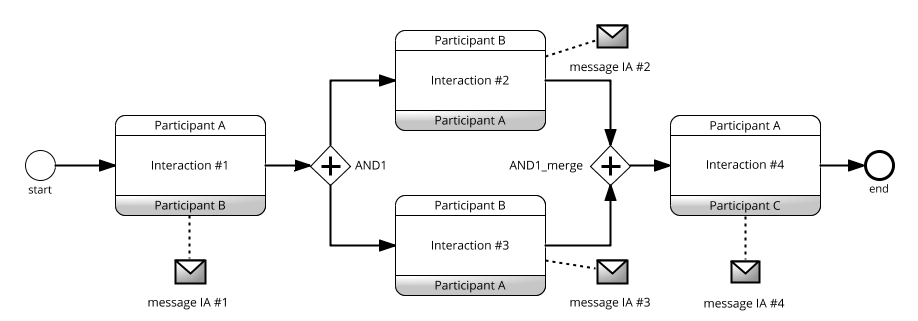
\includegraphics[width=1\textwidth]{src/images/choreo2bpmn.png}
\caption{BPMN/XML Translation Example - Choreography Model}
\label{fig:choreo2bpmn}
\end{figure}

The BPMN/XML shown in Example \ref{lst:choreobpmnex} represents the valid translation of the example choreography model shown in Figure \ref{fig:choreo2bpmn}. Independent from the model type, every BPMN/XML has the root element \textit{definitions} with the namespace and schema declarations. The actual model objects are located inside the \textit{choreography} element as already explained above. Because all different model types share a common xml structure convention and other models, e.g. collaboration models, can have more than one process described inside one BPMN/XML, data objects (e.g. messages) are located outside the actual process definitions, to be referenced by every including process. \\

\lstset{language=XML, morekeywords={definitions, encoding, xmlns, typeLanguage, targetNamespace, xsi:schemaLocation, message, id, name, choreography, isClosed, participant, messageFlow, messageRef, sourceRef, targetRef, choreographyTask, initiatingParticipantRef, incoming, outgoing, participantRef, messageFlowRef, startEvent, endEvent, parallelGateway, exclusiveGateway, gatewayDirection, sequenceFlow, sendTask, receiveTask, task}, basicstyle=\tiny, breaklines=true, frame=single}

\begin{lstlisting}[caption={BPMN Choreography Model Example},captionpos=b, label={lst:choreobpmnex}]
<?xml version="1.0" encoding="UTF-8"?>
<definitions xmlns="http://www.omg.org/spec/BPMN/20100524/MODEL" xmlns:xsi="http://www.w3.org/2001/XMLSchema-instance" typeLanguage="http://www.w3.org/2001/XMLSchema" xsi:schemaLocation="http://www.omg.org/spec/BPMN/20100524/MODEL http://www.omg.org/spec/BPMN/2.0/20100501/BPMN20.xsd"> 
  <message id="m111" name="message IA #1"/>
  <message id="m112" name="message IA #2"/>
  <message id="m113" name="message IA #3"/>
  <message id="m113" name="message IA #4"/>
  <choreography id="c111">
    <participant id="p111" name="Participant A"/>
    <participant id="p112" name="Participant B"/>
    <participant id="p113" name="Participant C"/>
    <messageFlow id="mf111" messageRef="m111" sourceRef="p111" targetRef="p112"/>
    <messageFlow id="mf112" messageRef="m112" sourceRef="p112" targetRef="p111"/>
    <messageFlow id="mf113" messageRef="m113" sourceRef="p112" targetRef="p111"/>
    <messageFlow id="mf114" messageRef="m113" sourceRef="p112" targetRef="p111"/>
    <choreographyTask id="ct111" name="Interaction #1" initiatingParticipantRef="p111">
      <incoming>sf111</incoming>
      <outgoing>sf112</outgoing>
      <participantRef>p111</participantRef>
      <participantRef>p112</participantRef>
      <messageFlowRef>mf111</messageFlowRef>
    </choreographyTask>
    <choreographyTask id="ct112" name="Interaction #2" initiatingParticipantRef="p112">
      <incoming>sf113</incoming>
      <outgoing>sf115</outgoing>
      <participantRef>p112</participantRef>
      <participantRef>p111</participantRef>
      <messageFlowRef>mf112</messageFlowRef>
    </choreographyTask>
    <choreographyTask id="ct113" name="Interaction #3" initiatingParticipantRef="p112">
      <incoming>sf114</incoming>
      <outgoing>sf115</outgoing>
      <participantRef>p112</participantRef>
      <participantRef>p111</participantRef>
      <messageFlowRef>mf113</messageFlowRef>
    </choreographyTask>
    <choreographyTask id="ct114" name="Interaction #4" initiatingParticipantRef="p111">
      <incoming>sf117</incoming>
      <outgoing>sf118</outgoing>
      <participantRef>p111</participantRef>
      <participantRef>p113</participantRef>
      <messageFlowRef>mf114</messageFlowRef>
    </choreographyTask>
    <startEvent id="e111" name="start">
      <outgoing>sf111</outgoing>
    </startEvent>
    <endEvent id="e112" name="end">
      <incoming>sf117</incoming>
    </endEvent>
    <parallelGateway id="g111" name="AND1" gatewayDirection="Diverging">
      <incoming>sf112</incoming>
      <outgoing>sf113</outgoing>
      <outgoing>sf114</outgoing>
    </parallelGateway>
    <parallelGateway id="g112" name="AND1_merge" gatewayDirection="Converging">
      <incoming>sf115</incoming>
      <incoming>sf116</incoming>
      <outgoing>sf117</outgoing>
    </parallelGateway>
    <sequenceFlow id="sf111" name="" sourceRef="e111" targetRef="ct111"/>
    <sequenceFlow id="sf112" name="" sourceRef="ct111" targetRef="g111"/>
    <sequenceFlow id="sf113" name="" sourceRef="g111" targetRef="ct112"/>
    <sequenceFlow id="sf114" name="" sourceRef="g111" targetRef="ct113"/>
    <sequenceFlow id="sf115" name="" sourceRef="ct112" targetRef="g112"/>
    <sequenceFlow id="sf116" name="" sourceRef="ct113" targetRef="g112"/>
    <sequenceFlow id="sf117" name="" sourceRef="g112" targetRef="ct114"/>
    <sequenceFlow id="sf118" name="" sourceRef="ct114" targetRef="e112"/>
  </choreography>
</definitions>
\end{lstlisting}

\subsection{Collaboration / Public / Private Models}

As mentioned in Chapter \ref{chap:theo}, in a collaborative scenario, the collaboration, public and private models share the same BPMN/XML structure, because in each of the model types, there is at least one interactive task (send / receive messages) and a corresponding message flow (sender, receiver and message) that must be described within the BPMN/XML. Each partner can also decide if they want to share the private tasks within the public model and therefore also in the collaboration model, that is essentially a combined view of all partners public models. Because of this, the three model types can comprise all the BPMN objects shown in Table \ref{tbl:collab2bpmn}.

\lstset{language=XML, morekeywords={definitions, encoding, xmlns, typeLanguage, targetNamespace, xsi:schemaLocation, message, id, name, choreography, isClosed, participant, messageFlow, messageRef, sourceRef, targetRef, choreographyTask, initiatingParticipantRef, incoming, outgoing, participantRef, messageFlowRef, startEvent, endEvent, parallelGateway, exclusiveGateway, gatewayDirection, sequenceFlow, sendTask, receiveTask, task}, basicstyle=\tiny, breaklines=true, frame=none}

\begin{table}[H]
\centering
\begin{tabular}{l|l}
\multicolumn{1}{c|}{\textbf{Internal Object}} & \multicolumn{1}{l}{\textbf{BPMN/XML Element}}     \\ \hline
Send Task & 
\begin{lstlisting}
<sendTask id="(unique-id)" name="(name)">
    <incoming>ref-to-sequenceFlow</incoming>
    <outgoing>ref-to-sequenceFlow</outgoing>
</sendTask>
\end{lstlisting} \\ \hline
Receive Task & 
\begin{lstlisting}
<receiveTask id="(unique-id)" name="(name)">
    <incoming>ref-to-sequenceFlow</incoming>
    <outgoing>ref-to-sequenceFlow</outgoing>
</receiveTask>
\end{lstlisting} \\ \hline
Private Task & 
\begin{lstlisting}
<task id="(unique-id)" name="(name)">
    <incoming>ref-to-sequenceFlow</incoming>
    <outgoing>ref-to-sequenceFlow</outgoing>
</task>
\end{lstlisting} \\ \hline
\end{tabular}
\caption{Mapping Collaboration Model to BPMN/XML}
\label{tbl:collab2bpmn}
\end{table}

\begin{figure}[H]
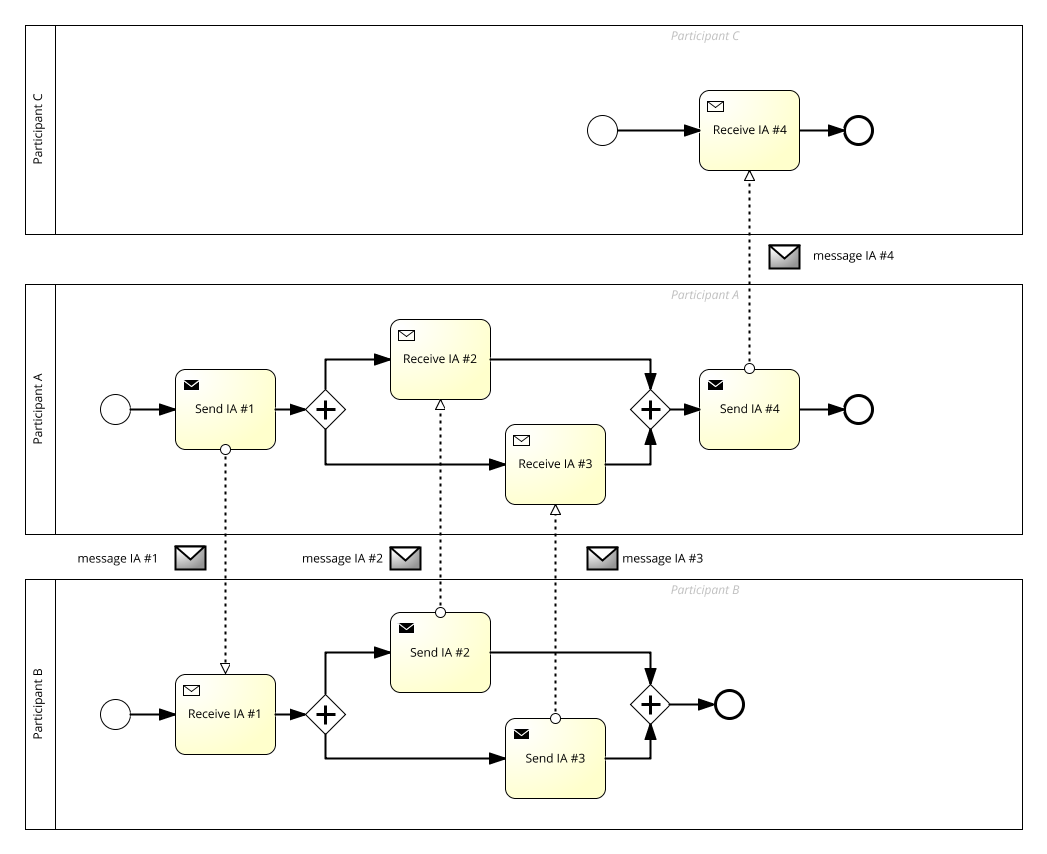
\includegraphics[width=1\textwidth]{src/images/collab2bpm.png}
\caption{BPMN/XML Translation Example - Collaboration Model}
\label{fig:collab2bpmn}
\end{figure}

The BPMN/XML shown in Example \ref{lst:collabbpmnex} represents the valid translation of the collaboration model shown in Figure \ref{fig:collab2bpmn}. Following the BPMN/XML convention, the root element is included as well the \textit{definitions} with the namespace and schema declarations. A layer below, the process independent data objects \textit{message}, the collaboration specific objects and a \textit{process} for each participant are defined. Within the \textit{collaboration} element, the participants, with a reference to their corresponding process and the message flow of the involving interacting tasks are declared. The \textit{messageFlow} object references the send and receive tasks that exchange the message. Or, if a process of a participant is represented as a black box, the \textit{messageFlow} object can also reference the process itself. In case of public or private models, where it is also possible that only one process of a specific participant is included, the \textit{messageFlow} object references the participant that sends or receives the message.

\lstset{language=XML, morekeywords={definitions, encoding, xmlns, typeLanguage, targetNamespace, xsi:schemaLocation, message, id, name, choreography, isClosed, participant, messageFlow, messageRef, sourceRef, targetRef, choreographyTask, initiatingParticipantRef, incoming, outgoing, participantRef, messageFlowRef, startEvent, endEvent, parallelGateway, exclusiveGateway, gatewayDirection, sequenceFlow, sendTask, receiveTask, task}, basicstyle=\tiny, breaklines=true, frame=single} 

\begin{lstlisting}[caption={BPMN Choreography Model Example},captionpos=b, label={lst:collabbpmnex}]
<?xml version="1.0" encoding="UTF-8"?>
<definitions xmlns="http://www.omg.org/spec/BPMN/20100524/MODEL" xmlns:xsi="http://www.w3.org/2001/XMLSchema-instance" typeLanguage="http://www.w3.org/2001/XMLSchema" xsi:schemaLocation="http://www.omg.org/spec/BPMN/20100524/MODEL http://www.omg.org/spec/BPMN/2.0/20100501/BPMN20.xsd">
   <message id="m1" name="message IA #1"/>
   <message id="m2" name="message IA #2"/>
   <message id="m3" name="message IA #3"/>
   <message id="m4" name="message IA #4"/>
   <collaboration id="collab1">
      <participant id="p1" name="Participant A" processRef="pr1"/>
      <participant id="p2" name="Participant B" processRef="pr2"/>
      <participant id="p3" name="Participant C" processRef="pr3"/>
      <messageFlow id="mf1" messageRef="m1" name="" sourceRef="t1" targetRef="t5"/>
      <messageFlow id="mf2" messageRef="m2" name="" sourceRef="t8" targetRef="t2"/>
      <messageFlow id="mf3" messageRef="m3" name="" sourceRef="t9" targetRef="t3"/>
      <messageFlow id="mf4" messageRef="m4" name="" sourceRef="t4" targetRef="pr3"/>
   </collaboration>
   <process id="pr1" name="Participant A">
      <sendTask id="t1" name="Send IA #1">
         <incoming>sf1</incoming>
         <outgoing>sf2</outgoing>
      </sendTask>
      <startEvent id="e1" name="start">
         <outgoing>sf1</outgoing>
      </startEvent>
      <parallelGateway gatewayDirection="Diverging" id="g1" name="AND1">
         <incoming>sf2</incoming>
         <outgoing>sf3</outgoing>
         <outgoing>sf4</outgoing>
      </parallelGateway>
      <receiveTask id="t2" name="Receive IA #2">
         <incoming>sf3</incoming>
         <outgoing>sf5</outgoing>
      </receiveTask>
      <receiveTask id="t3" name="Receive IA #3">
         <incoming>sf4</incoming>
         <outgoing>sf6</outgoing>
      </receiveTask>
      <sendTask id="t4" name="Send IA #4">
         <incoming>sf7</incoming>
         <outgoing>sf8</outgoing>
      </sendTask>
      <parallelGateway gatewayDirection="Converging" id="g2" name="AND1_merge">
         <incoming>sf5</incoming>
         <incoming>sf6</incoming>
         <outgoing>sf7</outgoing>
      </parallelGateway>
      <endEvent id="e2" name="end">
         <incoming>sf8</incoming>
      </endEvent>
      <sequenceFlow id="sf1" name="" sourceRef="e1" targetRef="t1"/>
      <sequenceFlow id="sf2" name="" sourceRef="t1" targetRef="g1"/>
      <sequenceFlow id="sf3" name="" sourceRef="g1" targetRef="t2"/>
      <sequenceFlow id="sf4" name="" sourceRef="g1" targetRef="t3"/>
      <sequenceFlow id="sf5" name="" sourceRef="t2" targetRef="g2"/>
      <sequenceFlow id="sf6" name="" sourceRef="t3" targetRef="g2"/>
      <sequenceFlow id="sf7" name="" sourceRef="g2" targetRef="t4"/>
      <sequenceFlow id="sf8" name="" sourceRef="t4" targetRef="e2"/>
   </process>
   <process id="pr2" name="Participant B">
      <startEvent id="e3" name="start">
         <outgoing>sf9</outgoing>
      </startEvent>
      <receiveTask id="t5" name="Receive IA #1">
         <incoming>sf9</incoming>
         <outgoing>sf10</outgoing>
      </receiveTask>
      <parallelGateway gatewayDirection="Diverging" id="g3" name="AND1">
         <incoming>sf10</incoming>
         <outgoing>sf11</outgoing>
         <outgoing>sf12</outgoing>
      </parallelGateway>
      <sendTask id="t6" name="Send IA #2">
         <incoming>sf11</incoming>
         <outgoing>sf13</outgoing>
      </sendTask>
      <sendTask id="t7" name="Send IA #3">
         <incoming>sf12</incoming>
         <outgoing>sf14</outgoing>
      </sendTask>
      <parallelGateway gatewayDirection="Converging" id="g4" name="AND1_merge">
         <incoming>sf13</incoming>
         <incoming>sf14</incoming>
         <outgoing>sf15</outgoing>
      </parallelGateway>
      <endEvent id="e4" name="end">
         <incoming>sf15</incoming>
      </endEvent>
      <sequenceFlow id="sf9" name="" sourceRef="e3" targetRef="t5"/>
      <sequenceFlow id="sf10" name="" sourceRef="t5" targetRef="g3"/>
      <sequenceFlow id="sf11" name="" sourceRef="g3" targetRef="t6"/>
      <sequenceFlow id="sf12" name="" sourceRef="g3" targetRef="t7"/>
      <sequenceFlow id="sf13" name="" sourceRef="t6" targetRef="t8"/>
      <sequenceFlow id="sf14" name="" sourceRef="t7" targetRef="t9"/>
      <sequenceFlow id="sf15" name="" sourceRef="t8" targetRef="g4"/>
   </process>
   <process id="pr3" name="Participant C">
   	<startEvent id="e5" name="start">
         <outgoing>sf16</outgoing>
   	</startEvent>
   	<receiveTask id="t8" name="Receive IA #4">
     	   <incoming>sf16</incoming>
         <outgoing>sf17</outgoing>
     	</receiveTask>
   	<endEvent id="e5" name="end">
         <incoming>sf17</incoming>
     	</endEvent>
      <sequenceFlow id="sf16" name="" sourceRef="t9" targetRef="g4"/>
      <sequenceFlow id="sf17" name="" sourceRef="g4" targetRef="e4"/>
   </process>
</definitions>
\end{lstlisting}

\section{Conclusion}
In this chapter, the followed \textit{top-down approach} of how to build a process collaboration, starting with the choreography model and then deriving the public and private models from it, was explained. It was also shown how the random choreography model generation can be influenced by specifying various build parameters as well as by imposing pattern-based compliance rules. Furthermore, all necessary components for generating sound choreography models that satisfy the three levels of correctness were introduced by explaining the involved generation algorithms as well as by pointing out the necessity of the \textit{Model Tracking} component, in which the model is decomposed into splits, branches and nodes. Also, the indispensability of the thereby involved control flow logic, with it's status model for branches and the necessary functionality of calculating the exact proportion of interactions that are at free disposal and those that have already determined places within the evolving model or those that will be needed later by paths that will be created by not yet consumed gateways, were highlighted. The chapter was concluded by explaining how the internal model representation is translated to BPMN/XML. Thereby, the mapping of the internal components to the corresponding BPMN/XML elements was shown.
In the next chapter, it will be explained how the introduced components of the random process collaboration generator are implemented within the CRISP framework.
\vspace{-0.5cm}
\chapter{Implementation}
\label{chap:impl}
As part of the C3Pro Project, a framework has been developed in JAVA to test the elaborated change negotiation and propagation algorithms for collaborative processes. The framework already provides functions for importing process models in form of BPMN 2.0 XML. Within this importing process, the BPMN models are converted into a framework internal graph representation without loosing any information about the control flow and connection objects of the original model. This resulting graph structure then enables modest model manipulation and analysis techniques.\par
In order to save the effort of implementing the same or at least a likewise graph model structure for the automatic process collaboration generator, it was decided to integrate it into the existing framework. Hence, the structure and it's complementary components and services can be utilized with minor adoptions.\par
The following chapters describe the internal process model representation structure, the algorithms and components of the implemented automatic generator as well as the translation algorithm to transfer the resulting models to BPMN 2.0 XML.

\section{Internal Process Model Representation}
The framework internal process model representation utilizes the jBPT\footnote{Business Process Technologies for Java - https://code.google.com/p/jbpt/} library, which was developed by Polyvyanyy et. al \cite{jbpt} in the context of their compendium of process technologies and facilitates the development of process models in JAVA. Figure \ref{fig:jbpt} shows an excerpt of the core structure of the library. The structure enables the creation of different types of graphs to support the capturing of various process modeling languages, such as petri nets, EPC\footnote{Event-driven process chains} or BPMN.\par
For the purpose of constructing BPMN process models, an implementation of the \textit{AbstractMultiDirectedGraph} class is suitable. A \textit{multi directed graph} represents a graph, whose vertices can be connected among themselves through more than one \textit{directed} edges\cite{graph_theory}. Figure \ref{fig:jbpt} also shows that all graph models are typed with generics. In the context of a \textit{multi directed graph} model, the parameter \textit{E} is bound to a an instance of \textit{IDirectedEdge\textless$V$\textgreater}, whereas parameter \textit{V} is bound to an instance of \textit{IVertex}. 

\begin{figure}[H]
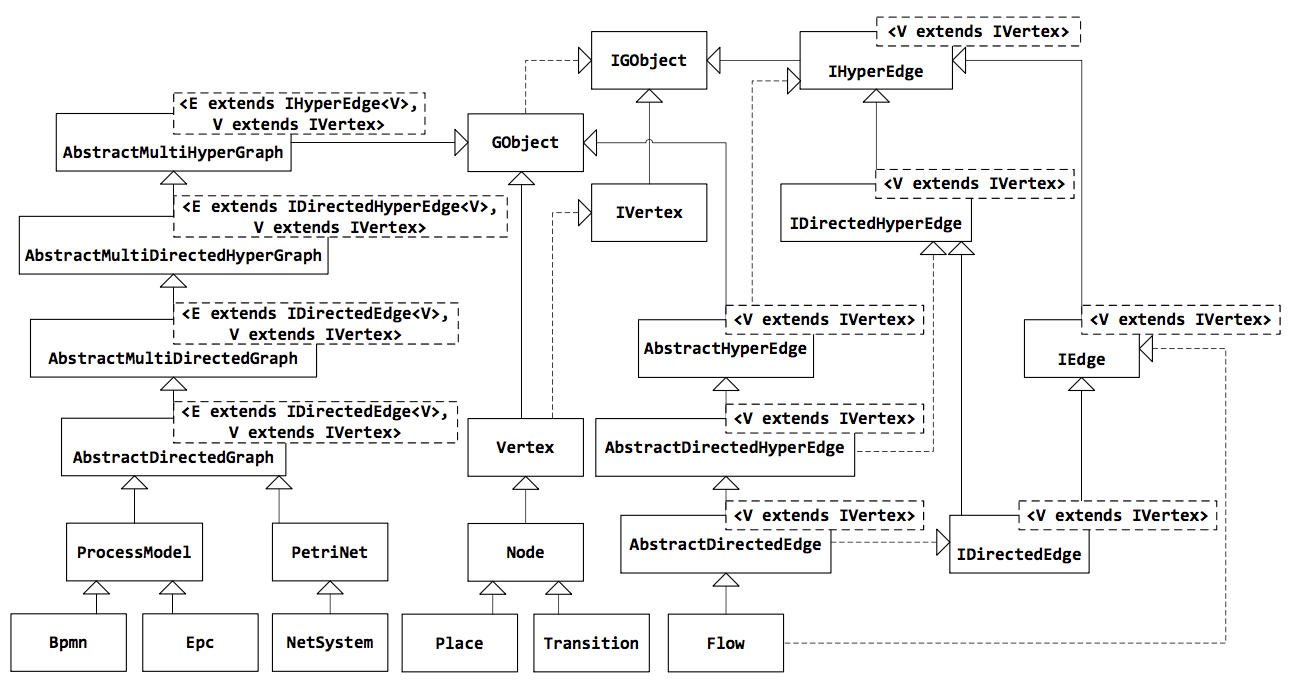
\includegraphics[width=1\textwidth]{src/images/class_diagram_jbpt.png}
\caption{Class and interface hierarchy of jBPT}
\label{fig:jbpt}
\end{figure}

In order to utilize the jBPT structure to build any type of BPMN process model, all specific BPMN flow objects, must therefor implement the \textit{IVertex} interface. The flow objects, for instance tasks or gateways, are then in turn connected through Edges, which represent the BPMN sequence flow, to create the graph and therefor the process model. How the jBPT library is incorporated and utilized by the C3Pro framework is illustrated in figure \ref{fig:choreo_structure}. 
The intensive use of interfaces, enables the reuse of flow objects, that are part of different model types. For instance, gateways and events are used in all four. For the sake of clarity, figure \ref{fig:choreo_structure} only shows model specific flow objects, that are appropriate for BPMN choreography models. Table \ref{tab:flow_objects} lists all BPMN flow objects, that are supported by the C3Pro framework to create process collaborations and their different models.\\

\begin{table}[H]
\resizebox{\textwidth}{!}
{
\begin{tabular}{l|cccc}
			      & Choreography Model & Collaboration Model & Public Model & Private Model \\ \hline
Start Event       & $\blacksquare$	  & $\blacksquare$      & $\blacksquare$	  & $\blacksquare$  \\
End Event         & $\blacksquare$	  & $\blacksquare$      & $\blacksquare$	  & $\blacksquare$  \\
Parallel Gateway  & $\blacksquare$    & $\blacksquare$      & $\blacksquare$      & $\blacksquare$  \\
Exclusive Gateway & $\blacksquare$    & $\blacksquare$      & $\blacksquare$      & $\blacksquare$  \\
Interaction       & $\blacksquare$    & $\square$           & $\square$           & $\square$       \\
Task          	  & $\square$         & $\blacksquare$      & $\blacksquare$      & $\blacksquare$  \\
Send Task         & $\square$         & $\blacksquare$      & $\blacksquare$      & $\blacksquare$  \\
Receive Task      & $\square$         & $\blacksquare$		& $\blacksquare$      & $\blacksquare$       
\end{tabular}%
}
\caption{Overview of supported BPMN flow objects}
\label{tab:flow_objects}
\end{table}

Within the C3Pro framework, all four model types support the flow objects \textit{start event, end event, parallel gateway} and \textit{exclusive gateway}. These are basic control flow objects, that are not specific to any model type in BPMN. Additionally available, for \textit{collaboration, public} and \textit{private models} are the activities \textit{Task, Send Task} and \textit{Receive Task}. According to the BPMN 2.0 specification, the activity \textit{task} represents an \textit{abstract task} \cite{BPMN20}. An \textit{abstract task} is a task that is not further specified. There are several further specified tasks in BPMN, including the also supported \textit{send} and \textit{receive task}. Since the focus of the C3Pro project is on collaborative processes and the message exchange between the participating partners, it's mandatory that these two messaging activities are also specified within the framework. For the remaining activities, that are not part of the message flow, it is in this context not relevant if the task is actually a \textit{user, manual, service} or \textit{script task}. The only flow object specific for \textit{Choreography Models} is the \textit{Choreography Task} or \textit{Interaction}, the equivalent of a \textit{send} and \textit{receive task} sequence in a collaboration model.   

\begin{figure}[H]
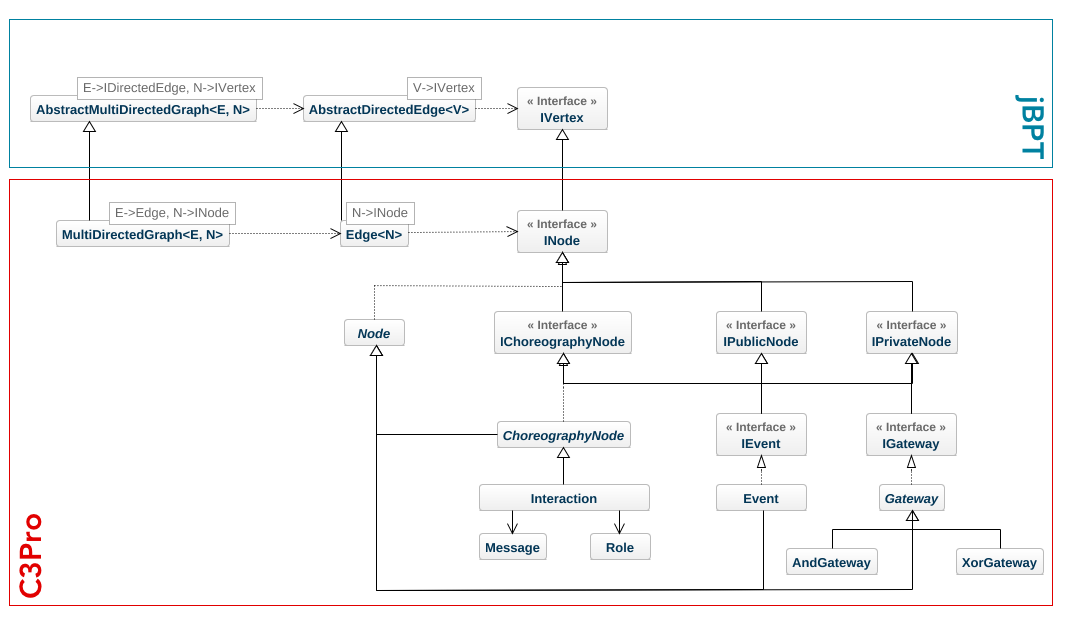
\includegraphics[width=1\textwidth]{src/images/c3pro_graph_structure.png}
\caption{C3Pro Model Representation Structure}
\label{fig:choreo_structure}
\end{figure}

\section{Approach}

As already mentioned in the chapter of theoretical background, a process collaboration between several partners can be modeled from different perspectives (partner or global) through the use of different model types. The process collaboration generator implemented in the context of this work, generates all four different model types as the outcome. In general, there exist two different approaches to build a process collaboration with all the described models \cite{sabrina1174}. At the \textit{top-down approach}, first the choreography model is build. Based on the choreography, then the public and private models of each partner are defined consistently. On the other hand, at the \textit{bottom-up approach}, each partner has already defined a private and public process. Then, the choreography model is constructed by connecting the public models via message exchange. \par
The automatic generator, presented in this work, follows the \textit{top-down approach}, by first generating the choreography model and then deriving the collaboration, public and private models from it. Thereby, each interaction (choreography task) of the choreography model, is converted into an send and receive task and then added to the involved partners processes, to build their public process models. Then in turn, each private model is derived from it's corresponding public model by enriching the public model with some abstract private tasks. The collaboration model is then build by compositing the partner's public processes into one model.\\

Generally, when defining business process models, three levels of correctness that build upon each other must to be considered and satisfied by the models: \\

\begin{wrapfigure}{r}{0.5\textwidth}
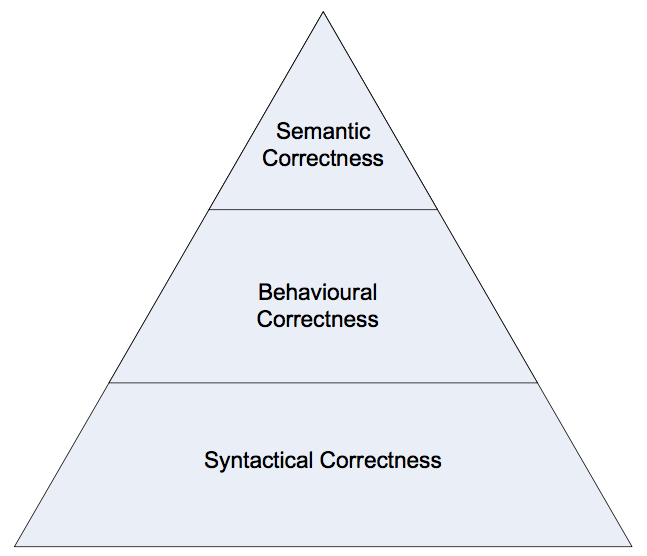
\includegraphics[width=0.9\linewidth]{src/images/correctness_levels.png}
\caption{Pyramid of Business Process Model Correctness}
\label{fig:bpm_correctness}
\end{wrapfigure}

\textit{Syntactical Correctness} is defined by the underlying BPMN meta model and refers to the correct use and composition of the corresponding model elements. Syntactical constraints for example include, that any model must have at least one start and one end event, as well as that flow objects (e.g. tasks, gateways, events) can only be connected by control flow edges \cite{sabrina848}. \\

\textit{Behavioral Correctness} constitutes that a process model must be executable and therefor to be free of deadlocks or lifelocks. It presumes that the model is syntactical correct, because the behavior of a syntactical incorrect model is undefined. Regarding collaborative, cross-organizational processes, it is also required that the composition of the involved public models are compatible. For example, this means, that for every message that is send, a corresponding partner must be able to receive it \cite{sabrina1174, sabrina848}. \\

\textit{Semantic Correctness} means that the a process model must comply with imposed compliance rules \cite{sabrina848}. Thereby it must be differentiated between \textit{local} and \textit{global compliance rules}. \textit{Local compliance rules} constrain the private process of a partners, whereas \textit{global compliance rules} constrain the interaction between multiple partners \cite{sabrina1174}. In this work, only \textit{global compliance rules} are imposed to constrain the choreography model. \\

All three levels of correctness are considered by the developed algorithm of the implemented automatic process generator. The algorithm ensures that only model specific flow objects are used to build the processes and that they are connected appropriately (syntactical correctness). It also guarantees the absence of deadlock and lifelocks (behavioral correctness) and offers the possibility to define global compliance rules (see next chapter), to which the generated collaboration complies to (semantic correctness). The introduced approach of deriving all models out of the before generated choreography model offers also the advantage, that if the deriving process is implemented correctly, it already ensures \textit{consistency} and \textit{compatibility} between the different models. In the context of collaborative processes, \textit{consistency} means, that the private model of a partner has to be consistent with the corresponding public model. This ensures that the executed business process of one partner satisfies the behavior that is communicated to the partners through his public models \cite{sabrina1174}. \\

\section{Constraining the Collaboration Generation}

Despite the premise, that the process collaborations should be generated randomly, it is reasonable to set some boundaries within the random generation takes place. The implemented generator provides two different ways to influence the resulting choreography model and hence the whole collaboration. The first one, provides the possibility to constrain the choreography model in terms of the employed flow objects and their exact quantity by specifying several input parameters. The second one, let the user impose global compliance rules based on compliance patterns to which the resulting model must comply to.

\subsection{Parametric Constraints} \label{sec:param_constraints}

Following input parameters are specified to influence the random generation of the choreography model and hence also the deriving models:

\begin{itemize}
\item Number of Partners
\item Number of Interactions
\item Number of Exclusive Gateways
\item Number of Parallel Gateways
\item Number of Loops
\item Max. Branching
\end{itemize}

\textit{Number of Partners} determines the number of participants which are involved in the process collaboration, whereas \textit{Number of Interactions} specifies the number of messages which are exchanged between the partners. \textit{Number of Exlusive/Parallel Gateways} in combination with \textit{Max. Branching} influences the the branching of the resulting process model. The First applies the exact number of the respective flow object into the model, whereas the second sets the upper boundary of branching (splitting the path) for each gateway. The lower boundary is set to two. Within this range, the generating algorithm determines a random number of following paths for each gateway placed into the model. This is explained in more detail later one. \textit{Number of Loops} determines the exact number of loops that should be placed into the model.

\subsection{Compliance Constraints}

Generally, compliance rules can be defined for different process flow perspectives of a process. It can be distinguished between compliance rules that constrain the control flow (sequence of activities), the data associated with the activities, the resources (specific user or role) that perform the activities or the time perspective. There exist several languages and approaches on how to define and specify compliance rules, including formal languages \cite{Ghose2007},\cite{GovMilSad:edoc:06:compliance}, visual languages \cite{sabrina953},\cite{Awad2008} and pattern-based approaches \cite{compliance_patterns}, \cite{Ramezani2012}. Both, visual and pattern-based approaches, aim at hiding formal details (e.g. temporal logic) and therefore simplifying the specification of compliance rules. \\

For the specification of compliance rules for the automatic process generator, the pattern-based approach of Turetken et. al. \cite{compliance_patterns} is utilized. In \cite{compliance_patterns} a repository of \textit{process control patterns} is introduced, which are high-level templates used to represent process properties which the process specification must satisfy. There are four different groups of patterns: 

\begin{itemize}
\item \textit{Order} patterns concern the sequencing of activities. For Instance, `\textit{Customer\_Inquiry} LeadsTo \textit{Offer}', is used to express that after a inquiry is send and received, an offer must be prepared and send.
\item \textit{Occurrence} patterns represent rules to address the existence of certain activities. For instance, `\textit{Check\_Credit\_Worthiness} Universal', is used to express that the activity must always occur when the process is executed. 
\item \textit{Resource} patterns constrain that certain activities must be performed by a specific user or group of users (role). For instance, `\textit{Approve\_Offer} PerformedBy \textit{Role Q}' constrains, that the activity must be assigned to a user who is part of the user group Q.    
\item \textit{Time} patterns are used to assign temporal rules to Order or Occurrence patterns. For instance, `\textit{Customer\_Inquiry} LeadsTo \textit{Offer} Within \textit{7(days)}' constrains, that an Offer has to be replied within seven days after an inquiry has been received. 
\end{itemize}

Because the generated process collaborations neglects the data, time and resource perspective and focuses solely on the control flow, only compliance rules that constrain the sequence of activities are possible to impose. Following process control patterns are supported to constrain the automatic generated choreography:

\begin{table}[H]
\centering
\resizebox{12cm}{!}
{
\begin{tabular}{l|l}
Pattern		      & Description  \\ \hline
P LeadsTo Q       & Interaction P must lead to Interaction Q	  	 \\
P Precedes Q      & Interaction Q must be preceded by Interaction P	  \\
P Universal  	  & Interaction P must always occur throughout execution \\
P Exists		  & Interaction P must be specified in process \\
\end{tabular}%
}
\caption{Overview of supported Compliance Patterns}
\label{tab:compl_patterns}
\end{table}



\section{Random Collaboration Generation Process}

The class diagram shown in figure \ref{fig:choreo_gen_structure} gives a simplified overview of all the components which are necessary for generating an entire process collaboration, starting with the generation of the choreography model to imposing compliance rules and finishing with deriving the public and private models. It also shows the major operations provided by every component. 

\begin{figure}[H]
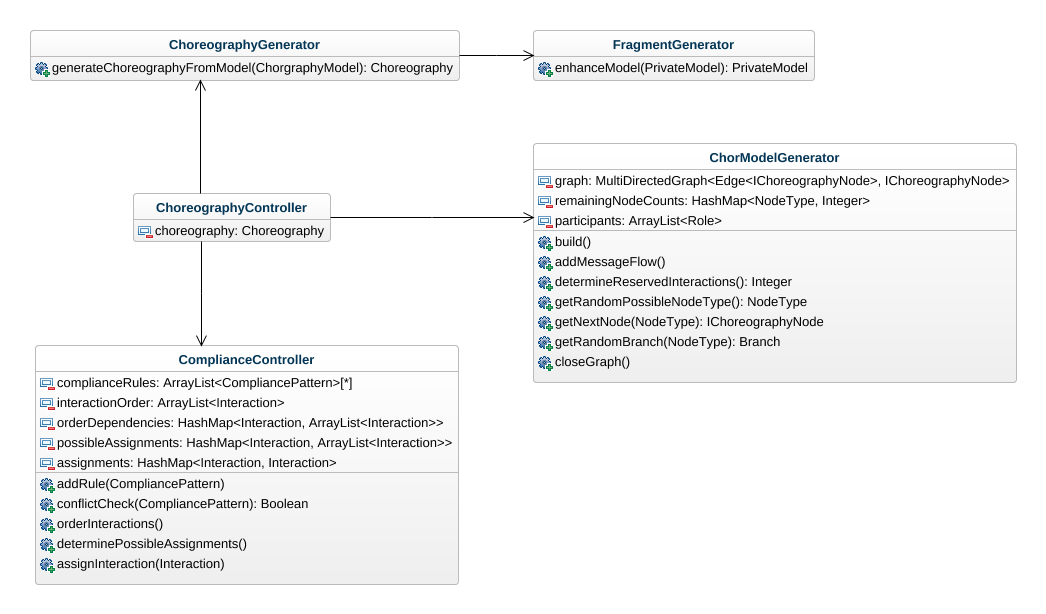
\includegraphics[width=1\textwidth]{src/images/ChorGen_Class.png}
\caption{Class Structure Choreography Model Generator}
\label{fig:choreo_gen_structure}
\end{figure}

In the following the components and their functionalities will be explained in detail.

\subsection{Choreography Controller}
The \textit{ChoreographyController} class represents the orchestration component for building random process collaborations, based on given constraints. The process follows the principle \textit{'first build then check'}, which means that after a random model has been generated, it will then be checked if the interactions defined within the compliance rules, can be assigned into the already built model in such a way that the resulting interaction sequence complies to the imposed rules. If the interaction allocation is not possible without violating the compliance rules, new random models will be build until a compliant model has been generated. Thereby the number of interactions will be increased by 10 percent every 10th build. After the successful assignment of the compliance rules, the remaining public and private models will be derived out of the generated choreography model. At last all models will be exported to a valid BMPN XML file. The whole process of generating a random choreography by coordinating the different functions is outlined with Algorithm \ref{alg:choreographyController}. \\

\begin{algorithm}[H]
\SetAlgoLined
\KwData{}
\KwResult{}
buildSuccess = \textbf{false}\;
\While{buildSuccess $\neq$ \textbf{true}}{
	build new choreography model\;
	\eIf{compliance rules are defined}{
		assign interactions\;
		\uIf{assignment successful}{
			buildSuccess = \textbf{true}\;
		}\ElseIf{number of interaction $\bmod$ 10 $\equiv$ 0}{
			increase number of interactions by factor 1.1\;
		}

	}{
		buildSuccess = \textbf{true}\;
	}
}
generate choreography\;
export models to BPMN\;
\caption{How to write algorithms}
\label{alg:choreographyController}
\end{algorithm}

\subsection{Choreography Model Generator}
The actual algorithm for generating graphs, representing choreography models, is implemented within the \textit{ChoreographyModelGenerator} component. Throughout the graph building process, it is essential to keep track of the current graph state at every point, in order to know where in the graph it is possible to put a new node without violating the syntactical correctness of the resulting BPMN model.  
Therefore a data model and corresponding logic is introduced in the \textit{GraphTracking} component, 
wherein the model is broken down into \textit{splits}, \textit{branches} and \textit{nodes}. A split is created for every gateway fork, that is put into the model. Every split has several branches (minimum two and maximum is defined by the max\_branching parameter), 
which are representing the different paths created by an parallel or exclusive gateway.    
Each branch holds the set of nodes that are on the path of this branch, whereas a path is limited by the merge node of it's corresponding fork gateway (split). In terms of a choreography model, nodes are limited to interactions and gateways.

\begin{figure}[H]
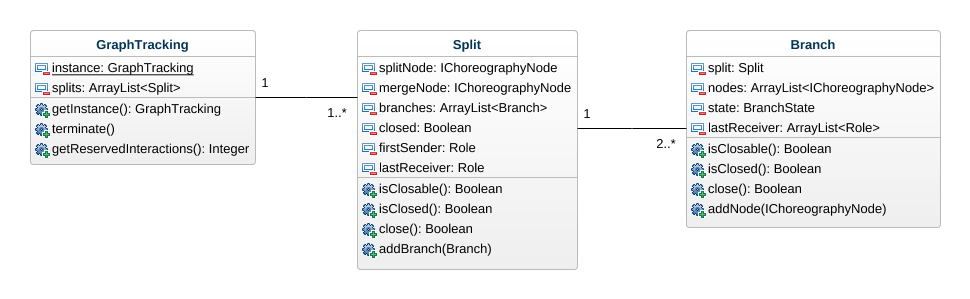
\includegraphics[width=1\textwidth]{src/images/graphtracking_cd.png}
\caption{Datamodel GraphTracking}
\label{fig:graphTracking2}
\end{figure}

Figure \ref{fig:graphTracking1} illustrates the concept of the \textit{GraphTracking} component. In this example, there are in total three splits with the split nodes: start event (blue), exclusive gateway\#1 (red) and parallel gateway \#1 (green). The split with the start event as the split node and the end event as the merge node has always only one branch, the main branch. Technically, this is not a split in the sense of the terminology. But because of the underlying data model, which is shown in figure \ref{fig:graphTracking2}, that defines that every branch must be related to a split, this pseudosplit is necessary to keep track of the main branch. The main branch (split \#1 - branch \#1) holds the set of ordered nodes: Interaction \#1, XOR gateway \#1, XOR merge \#1 and Interaction \#10.\\
Split \#2 has three branches. The first branch contains the nodes Interaction \#2 and Interaction \#5. The second branch consists only of Interaction \#3 and the third branch contains AND gateway \#1, AND merge \#1 and Interaction \#9. At last, the third split consists of two branches, which are holding the remaining interactions \#6, \#8 and \#7 respectively. 

\begin{figure}[H]
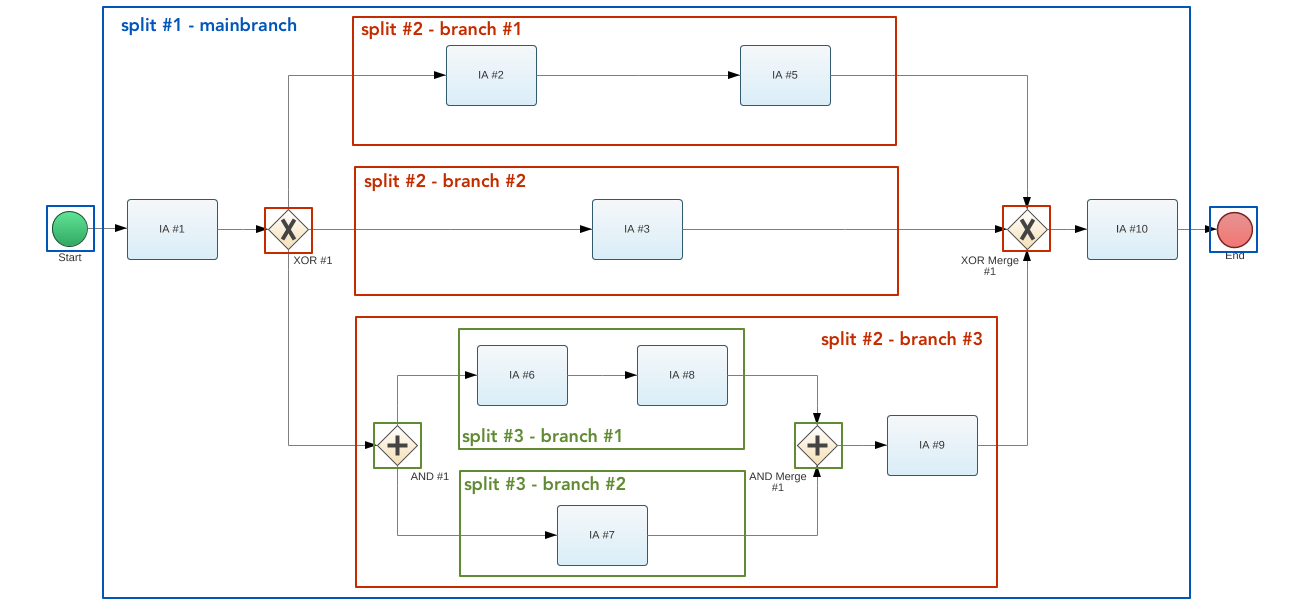
\includegraphics[width=1\textwidth]{src/images/graphTracking_1.png}
\caption{Concept of GraphTracking component}
\label{fig:graphTracking1}
\end{figure}

Furthermore, every split and every branch has a status. This status indicates whether the branch or split is \textit{open} or \textit{closed}. In case of a branch, open defines, that the branch is not yet enclosed by the merge node of it's corresponding split node and can further evolve by putting more nodes on its path. In turn, closed defines, that the branch is already finished by a connection of the last node with the respective merge node. A split is marked as closed, if all its branches are connected with the corresponding merge node, thus are closed. Additional to these two status, a branch can also be in the state \textit{split}. A branch has the state \textit{split}, if it contains a split and none of this split's branches are yet closed, thus there exists no merge node for this split. In this case, a branch can not evolve until one of it's enclosed branches is in state \textit{closed} and a merge node is placed on the split branch. Then the state changes from \textit{split} to \textit{open}. For example, in figure \ref{fig:graphTracking3}, the branch \#1 of split \#2 represents a branch in state \textit{split}, whereas the mainbranch is in state \textit{open} because branch \#2 of split \#1 is already closed by the merge node of split \#2.\\
During the build process it is also necessary to determine if a branch is allowed to be closed, without violating the soundness of BPMN choreography models. A branch is marked as closable, if there is an interaction on all it's enclosed paths. This approach of tracking the status of the branches becomes crucial the less remaining interactions are available and the more branches are still open in the model. Because of the parametric limitation of the number of interactions, at a certain point in the build process, not every open branch is allowed to be randomly selected for placing the next interaction or gateway without resulting in violating the correctness of the model or exceeding the number of interactions. In order to determine if this situation applies to a current point in a build process, the \textit{GraphTracking} component monitors the amount of \textit{free interactions} and \textit{reserved interactions}. 

\begin{figure}[H]
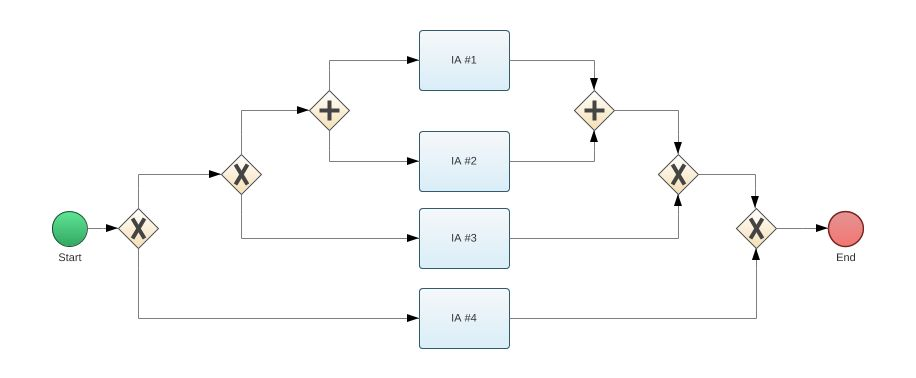
\includegraphics[width=1\textwidth]{src/images/proof_interactions.jpeg}
\caption{Minimum Interactions reserved by remaining gateways}
\label{fig:graphTracking4}
\end{figure}

Reserved interactions, are a certain amount of the remaining interaction that have either predetermined positions in the current graph (resInteractionsBranches) or will be needed in further paths created by not yet employed gateways (resInteractionsGateways). The exact amount of these reserved interactions, is depending on the number of not closable branches of the current graph and the number of gateways, that are not yet put into model. Regarding the current model, each open and non closable branch, increases the amount of \textit{resInteractionsBranches} by one. Gateways, that are not yet placed into the graph, will later create at least two new branches, that then again need at least one interaction on each of it's paths. Considering that a gateway node is allowed to be immediately followed by another gateways node without an interaction in between, the minimum amount of \textit{resInteractionsGateways} is $remaining gateways$ + 1. This influence of nested gateways onto the minimum amount of reserved interactions is illustrated in figure \ref{fig:graphTracking4}. After the amount of reserved interactions is calculated, the number of free interactions is determined by the difference between the amount of remaining interactions and the number of reserved interactions (see also definition \ref{def:def1}). If the amount of \textit{free interactions} $\equiv$ 0 then the random selection of the position in the graph is limited to the branches that are not yet closable, hence have not yet an interaction on their path. On the other hand, if the amount of \textit{free interactions} $\>$ 0, then all open branches can be selected for putting the next node.

\begin{Def}
	Let $x$ be the number of branches which are open and not closable, \\$remainingInteractions$ all the interactions not yet put into the model and \\$remainingSplits$ all the number of splits not yet put into the model. Then
	\begin{center}
		\textbf{resInteractionsBranches} = x\\
		\textbf{resInteractionsGateways} = $remainingSplits$ + 1\\
		\textbf{resInteractionsTotal} = $resInteractionsModel$ + $resInteractionsGateways$\\
		\textbf{freeInteractions} = $remainingInteractions$ - $reservedInteractionsTotal$
	\end{center}
	\label{def:def1}
\end{Def}


\begin{figure}[H]
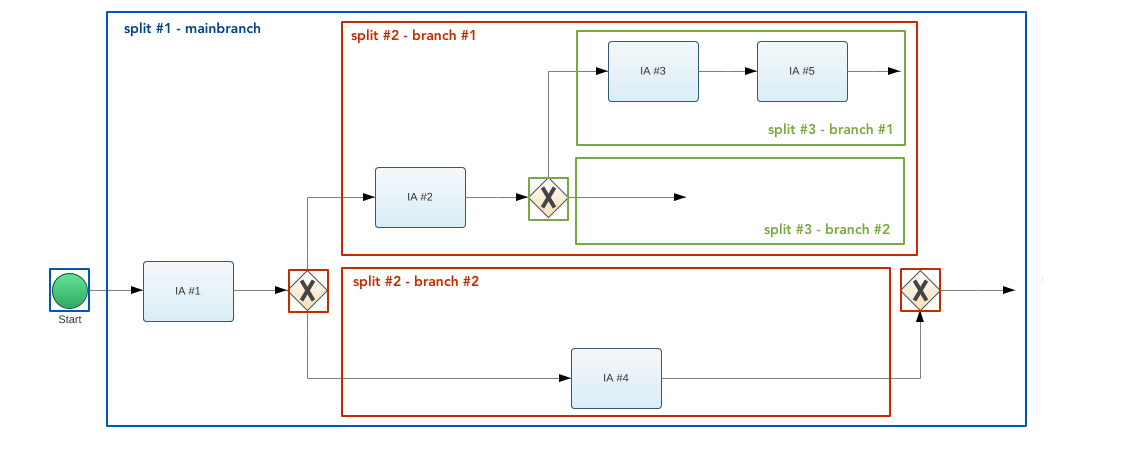
\includegraphics[width=1\textwidth]{src/images/graphTracking_status.png}
\caption{Minimum Interactions reserved by remaining gateways}
\label{fig:graphTracking3}
\end{figure}

Assuming a model generation where the total number of interactions being 6 and the total number of gateways being 2, the unfinished model in figure \ref{fig:graphTracking3} shows a choreography model at the point during the build process where not all open branches are allowed to be selected for placing the node (in this case an interaction). In order to obtain a sound choreography model while not increasing the number of initially specified interactions, the sixth interaction is only allowed to be placed on branch \#2 of split \#3. In this scenario, \textit{reservedInteractions} equals to one and \textit{freeInteractions} therefor equals to zero. On the other hand, if assuming the total number of interactions being 7, all branches of split \#3 and the mainbranch are possible candidates for placing the sixth interaction, because at this point, \textit{freeInteractions} would equal to one. \\

\begin{algorithm}[H]
\DontPrintSemicolon
\SetAlgoLined
\SetKwInOut{Input}{Input}\SetKwInOut{Output}{Output}
\Input{ 
\begin{itemize}[label={--}]
\setlength\itemsep{0em}
\item $remainingNodes \leftarrow$ number of nodes by type
\item $participants \leftarrow$ number of participants
\item $loops \leftarrow$ number of loops
\end{itemize}
}
\SetKwProg{Fn}{Function}{}{}
\SetKw{Continue}{continue}
\Begin{
	\If{number of interactions $\leq$ number of gateways + 1}{
		model generation is not possible\;
	}
	$graphTracking \leftarrow$ initialize GraphTracking\;
	\While{$remainingInteractions > 0$}{ 
		$nextNodeType \leftarrow$ getRandomNodeType()\;
		$selectedBranch \leftarrow$ getRandomBranch()\;
		\eIf{$selectedBranch$ is closable}{
			close branch by random\;
			\If{closed}{
				\Continue
			}
		}{
			$nextNode \leftarrow$ instantiate node of $nextNodeType$\;
			\If{$nextNodeType$ is gateway}{
				$branchCount \leftarrow$ getRandomBranchCount()\;
				$split \leftarrow$ instantiate new split\;
				$graphTracking.splits \leftarrow$ split\; 
				\For{$i \leftarrow$ 0 $branchCount$}{
					$branch \leftarrow$ instantiate new branch\;
					$split.branches \leftarrow branch$\;
					$i \leftarrow i$ + 1\;
				}
				add split and branches to SplitTracking\;
			}
			$selectedBranch.nodes \leftarrow$ $selectedBranch.nodes \cup nextNode$\;
			decrease $remainingNodes$ of $nextNodeType$\;
		}
	}
	close still open splits\;
	add end event to main branch\;
	enrich interactions with reasonable sender and receiver sequence\;
}
\caption{Generate Choreography Model}
\label{alg:choreoGen}
\end{algorithm}
\pagebreak
The actual procedure of generating random choreography models is shown in algorithm \ref{alg:choreoGen}. The input for a random model generation are the parametric constraints introduced in section \ref{sec:param_constraints}. At first, it is checked if the specified combination of the amount of interactions and gateways are sufficient to generate a sound model. This is the same evaluation as in determining the reserved interactions by remaining gateways. Therefore, the amount of interactions must be $\geq$ the amount of gateways + 1. If the validation is successful, the GraphTracking component gets instantiated. Thereby a split for the start event and the mainbranch is created. After GraphTracking is set up successfully, the algorithm loops over the number of remaining interactions until all interactions are put into the model. Within each loop, at first a node type for the next node is randomly selected out of the pool of remaining nodes. This can be an interaction, exclusive or parallel gateways depending on the number of free and reserved interactions. If there are free interactions available, the node type interaction is always in the pool of possible next node types. In case there are no free interactions left, the node type interaction will only get included in the possible next node types if not all remaining interactions are reserved by not yet consumed gateways. The algorithm for random possible node type selection is shown in \ref{alg:randNodeType}.\\

\begin{algorithm}[H]
\DontPrintSemicolon
\SetAlgoLined
\Begin{
	possibleNodeTypes $\leftarrow$ \{\}\;
	\If{freeInteractions $>$ 0 $\lor$ remInteractions $>$ resInteractionsGateways }{
		possibleNodeTypes $\leftarrow$ possibleNodeTypes $\cup$ Interaction\;
	}
	\If{remainingParallelGateways $>$ 0}{
		possibleNodeTypes $\leftarrow$ possibleNodeTypes $\cup$ ParallelGateways\;
	}
	\If{remainingExclusiveGateways $>$ 0}{
		possibleNodeTypes $\leftarrow$ possibleNodeTypes $\cup$ ExclusiveGateways\;
	}
	\Return random NodeType of possibleNodeTypes\;	
}
\caption{getRandomNodeType()}
\label{alg:randNodeType}
\end{algorithm}

After a node type has been selected, a position in the model is determined for placing a node of the previously selected node type by randomly selecting a possible open branch. Which branches are in the pool of possible, selectable branches, is again depending on whether there are free interactions available or not. If there are free interactions left, all open branches are allowed to be selected, independent from the prior selected node type. This changes if there are no free interactions remaining. In this case, only all open are allowed to be considered for random selection if again, not all remaining interactions are reserved by not yet consumed gateways. Otherwise only branches that are closable are allowed to be included in the pool of possible branches. The algorithm for random possible branch selection is shown in \ref{alg:randBranch}.\\

\begin{algorithm}[H]
\DontPrintSemicolon
\SetAlgoLined
\Begin{
	possibleBranches $\leftarrow$ \{\}\;
	\eIf{freeInteractions $>$ 0 $\lor$ remInteractions $>$ resInteractionsGateways }{
		possibleBranches $\leftarrow$ all open branches\;
	}{
		possibleBranches $\leftarrow$ all not closable branches\;
	}
	\Return random Branch of possibleBranches\;	
}
\caption{getRandomBranch()}
\label{alg:randBranch}
\end{algorithm}

In the next step, the random selected branch is checked whether it's closable or not and if so gets closed by random. This doesn't apply to the mainbranch to make sure that there is always one branch where the model can further evolve. This step of random branch closing is necessary to obtain balanced choreography models regarding nested branches. If there is no random branch closing mechanism the resulting models would be very similar. A mechanism that closes branches whenever they are possible to close would only result in models with lesser nested branches whereas a mechanism that never closes branches would result in models that have highly nested branches. If the selected branch gets randomly closed, a merge node for this branches split is created and added to the enclosing branch. Additionally, in the data model of the corresponding split, the merge node gets noted in order to assure that the last nodes of the other branches of this split will get connected with the same merge node when they get closed. Finally the algorithm jumps back to the beginning of the loop and starts again with randomly selecting a possible node type for the next node to be placed in the model.\\
By the time a branch is not randomly closed, a node of the predefined node type gets instantiated. In case of an interaction, only the plain object without any sender, receiver or message gets instantiated. Is the selected node type a gateway, the number of branches is determined by randomly selecting a number between 2 and the current maximum branching amount. The upper boarder of the maximum branching amount is generally limited by the user specified max branching parameter. But again, due to the limitation of interactions, the specified maximum amount of branches can not be adducted as the upper boarder without considering the current amount of free interactions. If only the user specified upper branching boarder is adducted, there is a high chance that this results in an inconsistent model, because there are not enough interactions for all paths that are created. In order to prevent this, the possible upper limit is determined dynamically each time a gateway node is put into the model by taking the minimum branching amount, which is always two, and adding the amount of free interactions. The algorithm for random possible branch amount selection is shown in \ref{alg:randBranchAmount}.\\

\begin{algorithm}[H]
\DontPrintSemicolon
\SetAlgoLined
\SetKwInOut{Input}{Input}\SetKwInOut{Output}{Output}
\Input{ 
\begin{itemize}[label={--}]
\setlength\itemsep{0em}
\item $minBranching \leftarrow$ 2\;
\item $maxBranching \leftarrow$ user specified upper branch amount border\;
\item $freeInteractions \leftarrow$ number of currently free interactions
\end{itemize}
}
\Begin{
	$possibleMaxBranching \leftarrow$ minBranching + freeInteractions\;
	\eIf{possibleMaxBranching $>$ maxBranching}{
		$currentMaxBranching \leftarrow$ maxBranching\;
	}{
		$currentMaxBranching \leftarrow$ possibleMaxBranching\;
	}
	\Return random value between minBranching and possibleMaxBranching\;	
}
\caption{getRandomBranchAmount()}
\label{alg:randBranchAmount}
\end{algorithm}

After a random number of branches is determined, the gateway node is added to the assigned branch and the corresponding split and branches are instantiated within GraphTracking.\\
Finally the amount of the selected node type is decreased by one and the loop starts over with selecting a random node type for the next node to be put into the model.\\
After all interactions and thus also all gateways are put into the model, the loop ends and all still open branches are getting closed. Algorithm \ref{alg:finishModel} displays the function to close all still open branches, by looping the graph recursively. At this point, where the model doesn't evolve furthermore, a branch is closed if the belonging split has a merge node assigned. If this is not the case, a merge node is created, added to the corresponding branch and assigned to the split.\\

\begin{algorithm}[H]
\DontPrintSemicolon
\SetAlgoLined
\SetKwInOut{Input}{Input}\SetKwInOut{Output}{Output}
\Input{ 
\begin{itemize}[label={--}]
\setlength\itemsep{0em}
\item $mainSplit \leftarrow$ split of mainbranch\;
\end{itemize}
}
\SetKwProg{Fn}{Function}{}{}
\Begin{
	\ForEach{branch of split.branches}{
		\ForEach{node of branch.nodes}{
			\If{node is gateway}{
				$closeSplit(split)$\;
			}
		}
		\If{branch is open}{
			$branch.close()$\;
		}
	}
}
\Fn{branch.close()}{
	$split \leftarrow$ split of branch\;
	\eIf{split.mergeNode == null}{
		$mergeNode \leftarrow$ instantiate merge node of gateway type\;
		$split.mergeNode \leftarrow$ mergeNode\;
		$branch.state \leftarrow$ closed\;
	}{
		$branch.state \leftarrow$ closed\;
	}
}
\caption{closeSplit(Split)}
\label{alg:finishModel}
\end{algorithm}

At this point the generated model is already syntactical correct because all model elements are used and connected according to BPMN specification. To achieve also behavioral correctness in choreopraphy models, beside a correct sequence flow, a message flow must be incorporated. Therefor, a sender and receiver must be assigned to each interaction forming a valid message sequence. To achieve a valid sender-receiver sequence, it must be taken into account, that the sender of an succeeding interaction Q must always be either the sender or receiver of the directly preceding interaction P on the path. If this rule is not considered and the sender of a succeeding interaction Q is neither the sending nor the receiving participant of the preceding interaction P, a flawless execution of the process is not possible, because the sender of interaction Q will never know if the preceding interaction P has been perfomed yet. In case of gateways, additionally it must be ensured, that the receiver of the last interaction of each branch of the gateway, is the same in order to determine a possible common sender for the succeeding interaction after the merge. Figure \ref{fig:messageFlow} illustrates a correct message flow within choreography models and algorithm xx describes the behaviour of the recursive function.  

\begin{figure}[H]
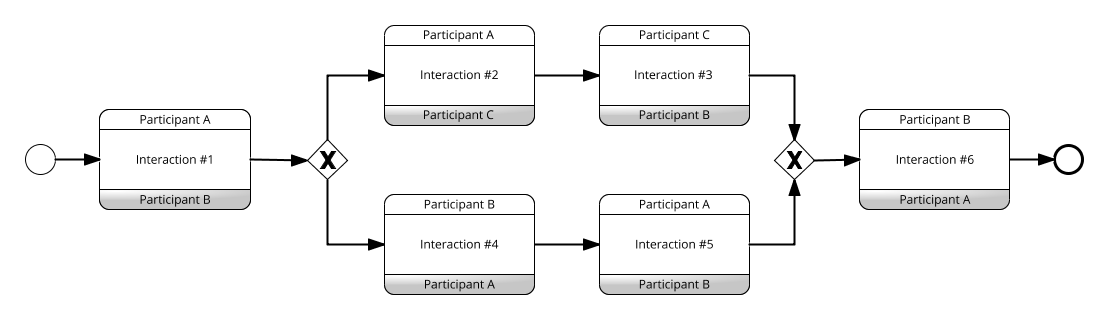
\includegraphics[width=1\textwidth]{src/images/messageFlow.png}
\caption{Message Flow - Sender/Receiver sequence}
\label{fig:messageflow}
\end{figure}

hier noch den algo einfügen bidde...\\
It should be noted, that because of the fact, that the sequence flow is first build without considering the corresponding message flow, it is likly that at some points an additional interaction must be inserted into the model to satisfy the above stated rules of sender-receiver sequences.


\subsection{ComplianceController}
As mentioned in the chapter of ChoreographyController, first a model is genereated and afterwards it is checked, if the interaction sequence specified within the compliance rules, can be applied to the generated model. Until now, the genereated model complies only to the parametric constraints. The logic of specifying and imposing compliance rules is implemented by the \textit{ComplianceController} component.\\

When specifying compliance rules to which the choreography model must comply to, it must be checked, if the imposed rules are consistent with one another. In the context of the four supported patterns (see xx), this applies only to the two order patterns (LeadsTo and Precedes). For instance, consider following set of compliance rules:

\begin{itemize}
\item \textit{CR-1}: P LeadsTo Q
\item \textit{CR-2}: Q LeadsTo S
\item \textit{CR-3}: S Precedes P
\end{itemize}

In this example, the rule \textit{CR-1} in combination with \textit{CR-2} is in conflict with \textit{CR-3}, because \textit{CR-1} and \textit{CR-2} determine, that the involved activities must occur in the order P-Q-S, whereas \textit{CR-3} constrains, that activity S must occur before activity P, which is in violation of the order determined by \textit{CR-1} and \textit{CR-2}. Algorithm \ref{alg:conflictCheck} demonstrates the conflict checking procedure implemented within the complicance controller component. \\

\begin{algorithm}[H]
\DontPrintSemicolon
\SetAlgoLined
\SetKwInOut{Input}{Input}
\SetKwInOut{Output}{Output}
\Input{ 
\begin{itemize}[label={--}]
\item compliance rule $cr$
\item dictionary $orderDependencies$ consisting of Interactions $P$ and their succeeding Interactions $S$
\end{itemize}
}

\SetKwProg{Fn}{Function}{}{}
\Begin{
	\If{$cr$ is order pattern}{
		$p \leftarrow$ preceding interaction of $cr$\;
		$s \leftarrow$ succeeding interaction of $cr$\;
		\eIf{!orderConflictCheck($p, s$)}{
			add $cr$ to $complianceRules$\;
			\eIf{$p \in P$ of $orderDependencies$}{
				add $s$ to succeeding interactions $S$ of $p$
			}{
				add $p$ to $orderDependencies$\;
				add $s$ to succeeding interactions $S$ of $p$ 
			}	
		}{
			add $cr$ to $conflictedRules$\;
		}
	}	
}
\Fn{orderConflictCheck($p, s$)}{
	\eIf{$s \in P$ of $orderDependencies$}{
		\ForEach{$s \in S$ of $p$}{
			\uIf{$s$ == $p$}{
				\Return \textbf{true}
			}\uElseIf{orderConflictCheck($s, p$)}{
				\Return \textbf{true}
			}
		}
	}{
		\Return \textbf{false} 	
	}
}
\caption{Add Compliance Rule}
\label{alg:conflictCheck}
\end{algorithm}

The result of this procdure is a set of conflict free compliance rules, that determine a specific order sequence between the involved interactions.
The specific interactions of the compliance rules are then tried to assign to the exisiting interactions within the before genereated model in a way that it complies to the interaction order and the compliance rules.


\subsection{ChoreographyGenerator}
This component is responsible for the process of deriving the public and private models of each participant from the before generated choreography model.


\section{Translator to BPMN/XML}

\vspace{-0.5cm}
\chapter{Performance Analysis}
\label{chap:analysis}
In this chapter, the influence of different build parameter settings on the performance of the generation process and the resulting choreography models is examined. As measure for the performance of a choreography generation process that is constraint by parametric constraints as well as imposed compliance rules (see Chapter \ref{sec:constraints}), the number of necessary iterations for a successful generation is adducted. The iteration limitation is thereby set to ten. After ten iterations, the choreography generation is marked as failed. For the examination of the generation process that is only constraint by parametric constraints, the necessary duration for a successful build is used as measure, because the generation algorithm ensures that a model generation without imposed compliance rule will always result in a successful model within one iteration. In the following, first, the performance dependent on the parametric constraints is analyzed, and afterwards, the influence of different compliance rule settings, in conjunction with parametric constraints, is examined. In order to obtain representative results, each parameter configuration is run with 100 repetitions, if not stated otherwise.\\

Figure \ref{fig:anal_gateways} illustrates the influence of the number of parallel gateways onto the duration of a choreography model generation with 100 interactions. It shows that the generation duration is increasing linear to the number of gateway nodes included in the model. It also shows that there is no significant difference between the respective gateway types and also the combination between parallel and exclusive gateways (equal proportion). The generation duration increase is expected, because the more gateways are in the model, the more branches are created, and the more branches are in the model, the longer it takes to loop through the model to determine the number of free or reserved interactions.\\

\begin{figure}[htb]
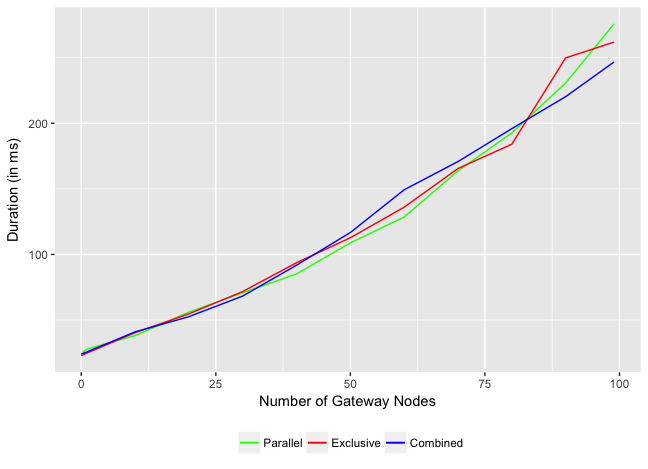
\includegraphics[width=1\textwidth]{src/images/analysis_gateways.png}
\caption{Choreography model generation duration depending on the number of gateway nodes}
\label{fig:anal_gateways}
\end{figure}

Figure \ref{fig:anal_branching} illustrates the influence of the max. branching parameter (see Section \ref{sec:param_constraints}) on the duration of a choreography model generation with 400 interactions and 20 gateway nodes. The graph shows that the generation duration is increasing linear to the increase of the max. branching parameter. The explanation for this is the same as for the influence of the number of gateway nodes. With the increase of the max. branching parameter, the number of branches in the build increases (premised that there are enough free interactions), and therefore the algorithms which loop through the branches consume more time.

\begin{figure}[htb]
\centering
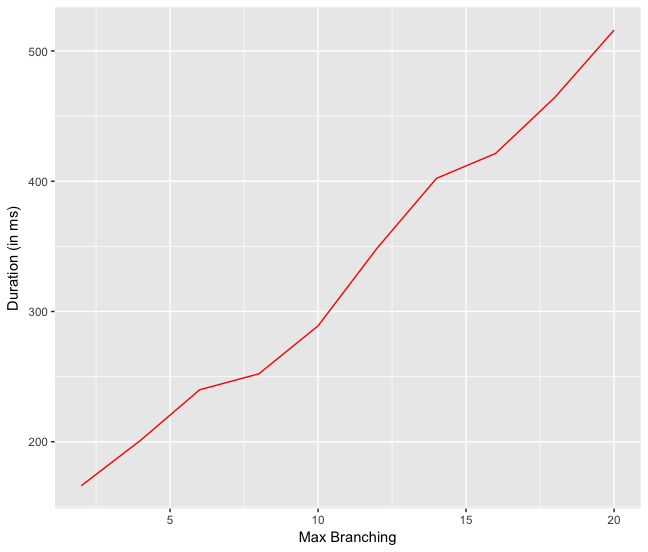
\includegraphics[width=0.9\textwidth]{src/images/analysis_branching.png}
\caption{Choreography model generation duration depending on the max. branching parameter}
\label{fig:anal_branching}
\end{figure}

For the analysis of the influence of different compliance rules settings on the model generation process, a random compliance rule generator is used. By specifying a number of interactions and a number of compliance rules, the generator generates supported compliance rules between those interactions randomly, which are then tried to be imposed on the generated models. Figure \ref{fig:anal_ands1} illustrates the influence of the number of compliance rules on a model generation process with 100 interactions, 10 parallel gateways and max. branching set to 2. It shows that the number of compliance rules has no impact on a model generation which only includes parallel gateways (various amounts of parallel gateway nodes were analyzed). Each model generation process was successful within the first iteration. This result is expected, because in a model without exclusive paths, all four supported compliance rule patterns (see Section \ref{sec:conception_compliance}), taken individually, can be assigned to any position in the model as long as they are one the same path (not parallel to another). 

\begin{figure}[htb]
\centering
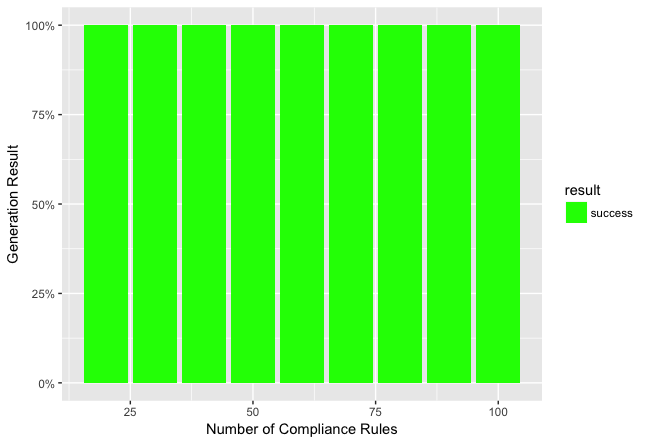
\includegraphics[width=0.9\textwidth]{src/images/ands_build_result.png}
\caption{Choreography model generation result depending on the number of compliance rules}
\label{fig:anal_ands1}
\end{figure}


This changes if a model generation includes exclusive gateways. Figure \ref{fig:anal_xors1} illustrates the influence of the number of compliance rules on a model generation process with 100 interactions, 10 exclusive gateways and max. branching set to 2. On the one hand, the result shows that the number of imposed compliance rule has no significant influence on the model generation success. On the other hand, on average only approx. 24\% of the generation processes are successful within 10 iterations. Figure \ref{fig:anal_xors2} shows the necessary iterations for the successful model generation processes depending on the number of specified compliance rules. This result is also expected, because the supported compliance rule patterns \textit{LeadsTo}, \textit{Precedes} and \textit{Universal} are hard to assign in a model with a lot of exclusive paths (see Definitions \ref{def:leadsto} - \ref{def:universal}). This is confirmed by examining the influence of the number of exclusive gateway onto a generation process restricted by 60 compliance rules, which is illustrated in Figure \ref{fig:anal_xors3}. The result shows that the more exclusive gateways, hence more exclusive paths, the more often the generation process fails within the specified iteration limitation. A successful generation is thereby also influenced by the level of dependency among the compliance rules. A high dependency among order patterns result in a more strict sequence order between the involved interactions, which makes it more difficult to assign them successfully.

\begin{figure}[htb]
\centering
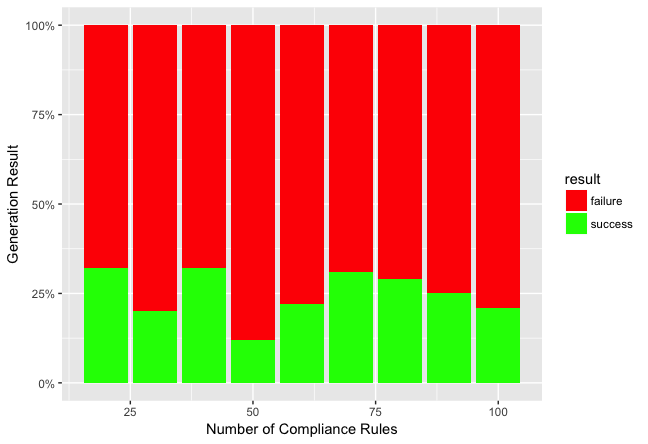
\includegraphics[width=0.9\textwidth]{src/images/xors_build_result.png}
\caption{Choreography model generation result depending on the number of compliance rules}
\label{fig:anal_xors1}
\end{figure}

\begin{figure}[H]
\centering
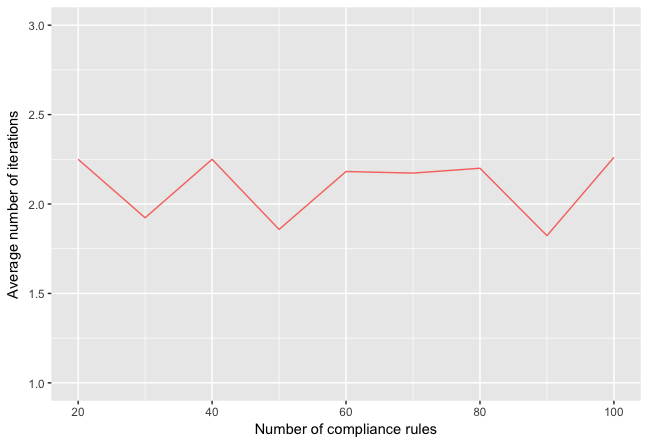
\includegraphics[width=0.9\textwidth]{src/images/xors_build_it.png}
\caption{Average iterations for successful generation}
\label{fig:anal_xors2}
\end{figure}

\begin{figure}[H]
\centering 
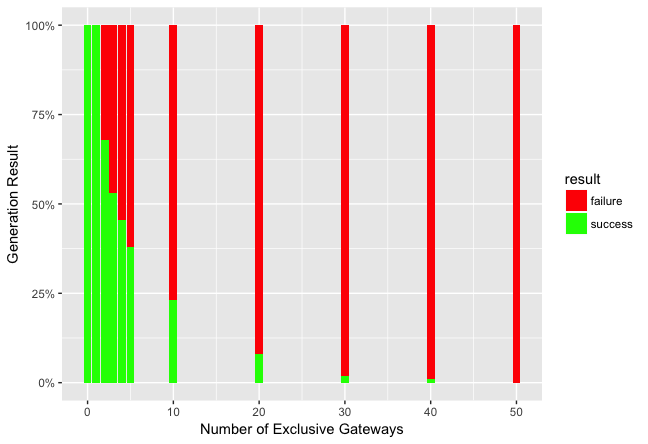
\includegraphics[width=0.9\textwidth]{src/images/xors_build_var.png}
\caption{Choreography generation result depending on the number of exclusive gateways and compliance rules}
\label{fig:anal_xors3}
\end{figure}


\vspace{-0.5cm}
\chapter{Conclusion and Future Work}
\label{chap:concl}
\section{Conclusion}
In this work, the lack of available collaborative process models represented in BPMN/XML for different research purposes, such as process mining or change propagation, was addressed. The main contribution within this work is the creation of a model repository by implementing a process generator which generates decentralized, cross-organizational models based on several, user-specified parameters. Thereby, an introduction into the two possible approaches of how to build collaborative processes, with all the models representing the different process perspectives, has been provided. It was argued that the followed \textit{top-down approach}, if implemented correctly, already provides good preconditions for ensuring compatibility between the public models as well as consistency between the public and the private model of one partner by deriving the public from the generated choreography model and enhancing the public model with private tasks to obtain the private model. Additionally to the model-specific parameters, also the possibility of specifying and imposing compliance rules was examined and evaluated by implementing a prototypical compliance rule component which supports a small subset of established compliance patterns in order to also examine the semantical correctness of the models. The main focus of this work was on the conception of the automatic generator and the therefor necessary components and algorithms. The benefit of expressing the models as a RPST was argued as well as the importance of tracking the model at any point during the generation process in order to comply with the user-specified parameters, which serve as boundaries for the random generation. Therefore, the \textit{Model Tracking} component and the concept of already reserved but not yet consumed interactions was explained in detail. Due to the simplicity of the underlying algorithms, the deriving and enhancement of the public and private model, as well as the translation of the internal model representation to BPMN/XML was merely discussed superficially by explaining the node mapping between the different models as well as the mapping to the BPMN/XML elements.\\
Finally, a performance analysis was performed, which showed the influence of different build parameters on the performance of the generation process as well as on the result. Thereby, it was shown that the number of specified nodes influences the performance of the generation process linearly. But the analysis also exposed room for improvement of the generation process in general and especially regarding the specification and imposition of compliance rules, which will be addressed in the next chapter.


\section{Future Work}
In the context of the conducted performance analysis, it was exposed that for generation processes with imposed compliance rules, combined with an amount of exclusive gateways greater than five, the outcome was not satisfying. By generating and imposing random compliance rules at a ratio of min. 1 : 5 to the amount of interactions, the build was only successful at approx. 1 out of 4 times. This was not unexpected and is a result of the characteristics of the supported compliance patterns, which are more difficult to assign the more they are interdependent. This problem could be solved by supporting more compliance patterns, especially \textit{P Exclusive Q}, which requires Interaction P to be on a different exclusive path than Interaction Q \cite{compliance_patterns}. In addition to that, the overall performance of assigning the compliance rules onto the model, could be improved by introducing a caching concept for possible positions instead of looping through the whole model for each compliance rule, which can be highly time consuming if the model is large. It would also be interesting for this problem to utilize a constraint solving framework like \textit{CHOCO}\footnote{An Open-Source java library for constraint programming - http://http://www.choco-solver.org/}. For the general build process, it could be conceivable to implement more parameters that allow the user to influence the model outcome even more. Thereby, for example, a parameter which influences the branch selection dependent on the degree of nested branching by dynamically favoring branches which are already highly nested or those that are not, depending on the parameter setting. 
\clearpage
\listoffigures
\listoftables
\clearpage
%---------------------------------------------------------
% bibliography based on Springer Design
%---------------------------------------------------------

\bibliographystyle{unsrt}
\bibliography{bibliography}
\clearpage
\appendix
\chapter{Appendix}
\section{Abstract}

In the research field of business process models and techniques, researchers can only rely on a repository of centralized, intra-organizational processes to use as support of their work. But regarding decentralized, cross-organizational models, they face the problem that there is a lack of available model examples. Within this work this lack is tried to be tackled. Thereby, a concept is introduced how to generate collaborative business processes randomly by following a \textit{top-down approach}, which first generates the choreography model and then derives the public and private models of each process participant from it. Additionally, a possibility for specifying and imposing global compliance rules onto the collaboration is elaborated. The conception of this random process generator is prototypically implemented within an existing framework in order to evaluate the process.

\section{Zusammenfassung}

Zur Unterstützung bei der Forschung an Geschäftsprozessmodellen und -techniken stehen lediglich ausreichend zentrale, unternehmensinterne Beispielprozesse zur Verfügung. Bei dezentralen, organisationsübergreifenden Prozessmodellen mangelt es allerdings an ausreichend verfügbaren Modellbeispielen. Im Rahmen dieser Arbeit wird versucht diesen Mangel zu beheben. Es wird ein Konzept vorgestellt, wie kollaborative Geschäftsprozesse randomisiert generiert werden können. Dabei wird ein "Top-Down" Ansatz verfolgt, der zunächst das Choreographie Modell generiert und anschließend die öffentlichen und privaten Modelle jedes Prozessteilnehmers daraus ableitet. Darüber hinaus wurde eine Möglichkeit erarbeitet, globale Compliance-Regeln zu definieren und dem Generierungsprozess als Rahmen aufzuerlegen. Um den erarbeiteten Prozess evaluieren zu können, wurde innerhalb eines bestehenden Frameworks ein Prototyp implementiert.



\printindex

\end{document}
